\documentclass[pdflatex,12pt]{aghdpl}
% \documentclass{aghdpl}               % przy kompilacji programem latex
% \documentclass[pdflatex,en]{aghdpl}  % praca w j�zyku angielskim
\usepackage[polish]{babel}
\usepackage[latin2]{inputenc}
% dodatkowe pakiety
\usepackage{enumerate}
\usepackage{listings}
\usepackage{caption}
\usepackage{multirow}
\usepackage{geometry}

\lstloadlanguages{TeX}

\newcommand{\degree}{\ensuremath{^\circ}}

%---------------------------------------------------------------------------

\author{�ukasz Mado�}
\shortauthor{�.Mado�}

\titlePL{Wizualizacja proces�w dyfuzji i porz�dkowania w stopach mi�dzymetalicznych}
%\titleEN{Visualisation of diffusion and ordering processes in intermetallic alloys}

\shorttitlePL{Wizualizacja proces�w dyfuzji i porz�dkowania w stopach mi�dzymetalicznych} % skr�cona wersja tytu�u je�li jest bardzo d�ugi
%\shorttitleEN{Visualisation of diffusion and ordering processes in intermetallic alloys}

\thesistypePL{Praca magisterska}
%\thesistypeEN{Master of Science Thesis}

\supervisorPL{dr Lucjan Pytlik}
%\supervisorEN{Lucjan Pytlik Ph.D}

\date{wrzesie� 2012}

\departmentPL{Katedra Informatyki Stosowanej i Fizyki Komputerowej}
%\departmentEN{Department of Applied Informatics and Computational Physics}

\facultyPL{Wydzia� Fizyki i Informatyki Stosowanej}
%\facultyEN{Faculty of Physics and Applied Computer Science}

%\acknowledgements{Serdecznie dzi�kuj� \dots tu ci�g dalszych podzi�kowa� np. dla promotora, �ony, s�siada itp.}



\setlength{\cftsecnumwidth}{10mm}

%---------------------------------------------------------------------------

\begin{document}

\titlepages

Merytoryczna ocena pracy przez opiekuna:
\clearpage
Merytoryczna ocena pracy przez recenzenta:
\clearpage

\rightline{Krak�w, wrzesie� 2012}
\begin{center}
{\bf Tematyka pracy magisterskiej i praktyki dyplomowej
�ukasza Madonia, studenta V roku studi�w kierunku informatyka stosowana, specjalno�ci informatyka
stosowana w nauce i technice}\\
\end{center}

Temat pracy magisterskiej:
{\bf Wizualizacja proces�w dyfuzji i porz�dkowania w stopach mi�dzymetalicznych.}\\

\begin{tabular}{rl}

Opiekun pracy:                  & dr  Lucjan Pytlik\\
Recenzenci pracy:               & dr hab. in�. Khalid Saeed\\
Miejsce praktyki dyplomowej:    & WFiIS AGH, Krak�w\\
\end{tabular}

\begin{center}
{\bf Program pracy magisterskiej i praktyki dyplomowej}
\end{center}

\begin{enumerate}
\item Om�wienie realizacji pracy magisterskiej z opiekunem.
\item Zebranie i opracowanie literatury dotycz�cej tematu pracy.
\item Praktyka dyplomowa:
\begin{itemize}
\item Zebrania wymaga� projektowych,
\item Wst�pna implementacja,
\item Projekt ostatecznej aplikacji
\item Implementacja i testy.
\end{itemize}
\item Opracowanie redakcyjne pracy.
\end{enumerate}


\noindent
Termin oddania w dziekanacie: wrzesie� 2012 \\[1cm]

\begin{center}
\begin{tabular}{lcr}
.............................................................. & ~~~ &
.............................................................. \\
(podpis kierownika katedry) & & (podpis opiekuna) \\
\end{tabular}
\end{center}

\tableofcontents
\clearpage

\chapter{Wprowadzenie}
\label{cha:wprowadzenie}
W dzisiejszych czasach komputer sta� si� niezb�dnym narz�dziem do rozwi�zywania problem�w wsp�czesnej fizyki. Fizyczne symulacje komputerowe s� naturalnym uzupe�nieniem fizyki teoretycznej oraz fizyki do�wiadczalnej. Mo�na w �atwy spos�b stworzy� abstrakcyjny model, kt�ry analizujemy lub poddajemy symulacji, w warunkach cz�sto nieosi�galnych do�wiadczalnie. Modele i symulacje komputerowe r�wnie� posiadaj� swoje wady, takie jak z�y zestaw za�o�e�, niewystarczaj�ca dok�adno��, zbyt kr�tki czas, dlatego te� trudnym wyzwaniem jest optymalne po��czenie do�wiadczenia i symulacji, tak aby uzyska� najlepsze wyniki. Jednym za zagadnie� fizycznych intensywnie badanych metodami komputerowymi jest wyt�umaczenie struktury i w�asno�ci z�o�onych stop�w metali - CMA. 

CMA (ang. Complex Metallic Alloys) definiuje si� jako stop metaliczny, posiadaj�cy kom�rk� elementarn� struktury krystalicznej, sk�adaj�c� si� z tysi�cy atom�w. Periodyczno�� kom�rki elementarnej jest znacznie wi�ksza ni� �rednia odleg�o�� pomi�dzy s�siadami w krysztale, przez co w�asno�ci fizyczne, a zw�aszcza transport elektron�w, r�ni� si� znacz�co od typowych kryszta��w. Istnieje kilka rodzaj�w CMA. Najintensywniej badane s� obecnie stopy oparte na aluminium, takie jak $\beta$- Mg$_{2}$Al$_{3}$\cite{CMAFund}.

Badanie struktury $\beta$- Mg$_{2}$Al$_{3}$  jest g��wnym powodem powstania omawianego programu do wizualizacji. Stop ten posiada wiele ciekawych w�asno�ci, takich jak niska g�sto��. Ponad jedna trzecia pozycji atomowych w siatce krystalicznej jest cz�ciowo obsadzona, co mo�e zosta� wykorzystane do magazynowania wodoru. lub materia� termoelektryczny. Interesuj�ce s� te� w�asno�ci termoelektryczne i wiele innych, kt�re nie zosta�y jeszcze do ko�ca zbadane\cite{SamRev}.
%---------------------------------------------------------------------------

\section{Cele pracy}
\label{sec:celePracy}

Celem pracy jest stworzenie, systemu pozwalaj�cego na wizualizacje proces�w dyfuzji i porz�dkowania w stopach mi�dzymetalicznych, takich jak stop $\beta$- Mg$_{2}$Al$_{3}$. Aplikacja b�dzie mia�a za zadanie obrazowanie zmian poziomu i typu obsadzenia w�z��w sieci krystalicznej. Zjawiska te s� na tyle uniwersalne w procesach transformacji, �e narz�dzie b�dzie mog�o znale�� zastosowanie przy analizie innych stop�w metali. Dodatkowo system b�dzie w stanie stworzy� klatki animacji, tak aby przedstawia�y one ewolucj� procesu. Oprogramowanie b�dzie u�ywane jako narz�dzie wspomagaj�ce prace fizyk�w. W pracy zawarty b�dzie r�wnie� opis struktur danych i algorytm�w u�ytych w aplikacji oraz proces jej projektowania. 

%---------------------------------------------------------------------------

\section{Zawarto�� pracy}
\label{sec:zawartoscPracy}

W rozdziale drugim opisz� z�o�one stopy metali, skupiaj�c si� g��wnie na $\beta$- Mg$_{2}$Al$_{3}$. Nast�pne rozdzia�y przynosz� informacj� na temat u�ytych algorytm�w oraz struktur danych. Postaram si� r�wnie� opisa� technologie, jakich u�y�em w kontek�cie wymaga� projektowych. Prac� zamyka rozdzia� po�wi�cony wnioskom z procesu realizacji programu. W pracy znajduje si� r�wnie� dodatek z instrukcj� obs�ugi. 



















\chapter{Zagadnienia fizyczne}
\label{cha:zagadnieniaTeoretyczne}
W danym rozdziale przedstawi� stan bada� do�wiadczalnych dotycz�cych w�asno�ci z�o�onych stop�w metali. Rozpoczn� od kr�tkiej charakterystyki struktur krystalicznych, tworzonych przez metale i ich stopy.

%---------------------------------------------------------------------------

\section{Z�o�one stopy metaliczne}
\label{sec:zlozoneStopyMet}

Metale i ich stopy w fazie sta�ej mog� tworzy� bardzo szerok� gam� struktur przestrzennych od dobrze uporz�dkowanych struktur krystalicznych a� do struktur ca�kowicie amorficznych. To w jakiej formie obserwujemy faz� sta��, zale�y w du�ym stopniu od historii obr�bki termicznej, czyli od tego, jak wolno dana substancja by�a sch�adzana. Mo�emy obserwowa� zar�wno dobrze uporz�dkowane fazy krystaliczne przy odpowiednio d�ugim wygrzewaniu, jak i szk�a metaliczne przy gwa�townym ch�odzeniu cieczy. Pomi�dzy tymi dwoma skrajno�ciami pojawi si� ca�a r�norodno�� faz cz�ciowo uporz�dkowanych i o r�nym poziomie defekt�w, takich jak wakancje, podmiany atom�w, dyslokacji i b��dy u�o�enia.
   
Wi�kszo�� czystych metali krystalizuje w jednej z trzech struktur krystalicznych, charakteryzuj�cych si� g�stym upakowaniem i du�� liczb� s�siad�w (l. koordynacyjn�). S� to struktury heksagonalne lub struktury regularne obj�to�ciowo (BCC) lub �ciennie (FCC) centrowane\cite{PhysRev}. W tej pracy bardziej b�d� nas interesowa� stopy metali, kt�re wykazuj� znacznie wi�ksze bogactwo zachowa�.

\begin{figure}[h!]
  \centering
	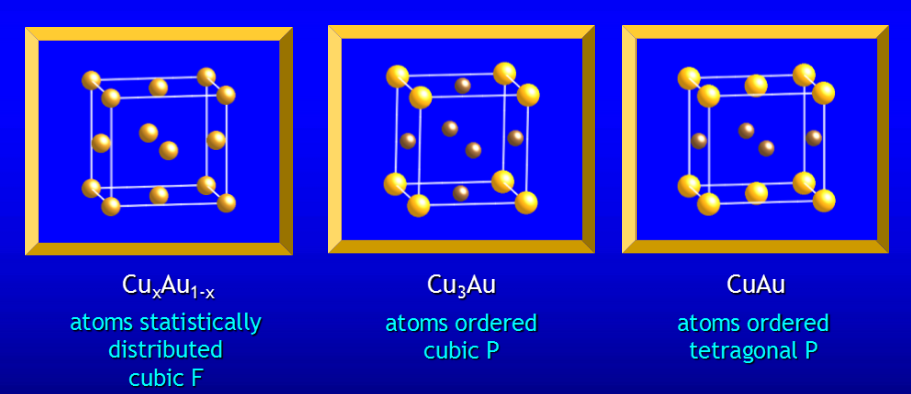
\includegraphics[scale=0.5]{hex}
	\caption{Uk�ady krystalograficzne dla stop�w $Au-Cu$, $AuCu$ i $Au_{3}Cu$.}
	\label{fig:hex}
\end{figure}

Stopy metali mo�emy podzieli� ze wzgl�du na ich struktur� wewn�trzn�. Rozr�niamy:
\begin{enumerate}%[1)]
\item roztw�r sta�y (w pewnym zakresie kompozycji), kiedy stop sk�ada si� z dw�ch pierwiastk�w (A i B), kt�re obsadzaj� zamiennie wsp�ln� sie� krystaliczn� (ka�dy w�ze� mo�e by� obsadzony przez atom A lub B). Mog� r�wnie� wyst�pi� atomy w pozycjach mi�dzyw�z�owych, przy wi�kszych r�nicach promieni atomowych. Po przekroczeniu granicy rozpuszczalno�ci otrzymujemy rozpad na mieszanin� r�nych faz. Zachowanie zale�y od regu�y Hume-Rothery. Przyk�adem jest stop miedzi i srebra (Cu-Ag).

\item stopy uporz�dkowane: kiedy po uporz�dkowaniu poszczeg�lne pozycje w sieci przyporz�dkowane s� danemu typowi atomu A lub B. Sie� krystaliczna pozostaje praktycznie taka sama, now� faz� daje tylko uporz�dkowanie obsadze�. Przyk�adem jest stop miedzi i z�ota(Cu-Au).

\item fazy po�rednie, w kt�rych przy okre�lonym zakresie kompozycji (blisko sk�adu idealnego) atomy tworz� faz� ze swoist� budow� krystaliczn�, nie zawsze b�d�c� w relacji z budow� krystaliczn� samych sk�adnik�w. 

\item zwi�zki mi�dzymetaliczne s� cz�stymi przedstawicielami faz z punktu 3, tych ze struktur� bardzo odmienn� od  struktury samych metali sk�adowych. Posiadaj� cechy, takie jak wi�zania w pe�ni izotropowe (metal), wysokie liczby koordynacyjne i du�a g�sto�� upakowania. Przyk�ady: fazy Lavesa, Heuslera, Franka-Kaspera, Zintla

\item z�o�one stopy mi�dzymetaliczne powstaj�, kiedy istniej� czynniki zak��caj�ce zbudowanie prostej struktury po�redniej fazy mi�dzymetalicznej. Mog� to by� relacje promieni atomowych, odej�cie od izotropowo�ci wi�za� lub pokrewie�stwo chemiczne. Efektem mo�e by� lokalne zak��cenie budowy prostej struktury i tworzenie klastr�w opartych na prostych relacjach geometrycznych i innych liczbach koordynacyjnych, np. fazy Samsona ($\beta$- Mg$_{2}$Al$_{3}$), Bergmana, Taylora. Obecno�� klastr�w powoduje trudno�ci ze wzajemnym wpasowaniem g��wnej fazy i element�w klastrowych, skutkuj�ce obecno�ci� wakancji, pozycjami mi�dzyw�z�owymi itd. Ta klasa ma wiele element�w wsp�lnych z kwazikryszta�ami. Bardzo wiele stop�w mi�dzymetalicznych jest kruchych w niskich temperaturach, jednak po osi�gni�ciu pewnej temperatury w�a�ciwo�ci fizyczne ulegaj� zmianie, przez co mo�na je zastosowa� w np. turbinie gazowej samolotu\cite{inter}.
\end{enumerate}

%Stop mi�dzymetaliczny jest to zwi�zek dw�ch lub wi�cej metali, kt�re s� powi�zane wi�zaniem metalicznym. 
%\begin{figure}[h!]
%  \centering
%	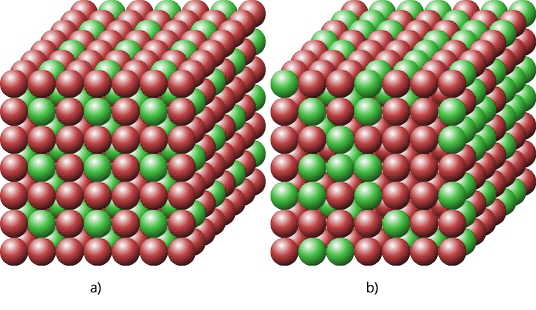
\includegraphics[scale=0.7]{Intermetallic}
%	\caption{Por�wnanie stop�w. a) stop mi�dzymetaliczny b) standardowy stop.}
%\end{figure}

%---------------------------------------------------------------------------

\section{Stop  $\beta$- Mg$_{2}$Al$_{3}$}
\label{sec:stopBetaMgAl}

Faza $\beta$- Mg$_{2}$Al$_{3}$ nale�y do najbardziej skomplikowanych w�r�d faz tego stopu. Odkrycia jej dokona� Riederer w 1936 roku na podstawie bada� dyfrakcyjnych\cite{Riederer}. Inny naukowiec, Perlitz, odkry�, �e stop sk�ada si� z 38\% magnezu i 62\% aluminium (wagowo). Posiada on r�wnie� kubiczn� grup� przestrzenn� Fd3m z kom�rk� elementarn� o boku r�wnym 2,822nm posiadaj�c� oko�o 1168 atom�w\cite{Perlitz}. G��wn� zalet� stopu $\beta$- Mg$_{2}$Al$_{3}$ jest bardzo ma�a g�sto�� i du�a liczba luk w sieci krystalicznej, co sugeruje mo�liwo�� ich wykorzystania jako akumulator�w wodoru\cite{PhysRev}. Rysunki \ref{fig:rzut} i \ref{fig:rzut2} przedstawiaj� przekr�j kom�rki elementarnej stopu $\beta$- Mg$_{2}$Al$_{3}$. Zielonym kolorem oznaczone s� atomy, kt�rych prawdopodobie�stwo obsadzenia wynosi 1 (stabilna siatka). Kolorem niebieskim oznaczona jest pozycja, w kt�rej istnieje mo�liwo�� obsadzenia atomem aluminium, natomiast kolor czerwony reprezentuje atom magnezu (cz�� klasterowa). 

\begin{figure}[h!]
  \centering
	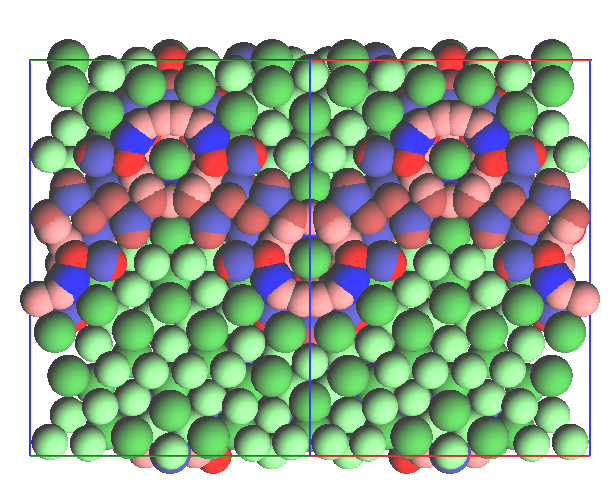
\includegraphics[scale=0.7]{rzut}
	\caption{Przekr�j kom�rki elementarnej $\beta$- Mg$_{2}$Al$_{3}$. P�aszczyzna prostopad�a do kierunku [1,1,0].}
	\label{fig:rzut}
\end{figure}

\begin{figure}[h!]
  \centering
	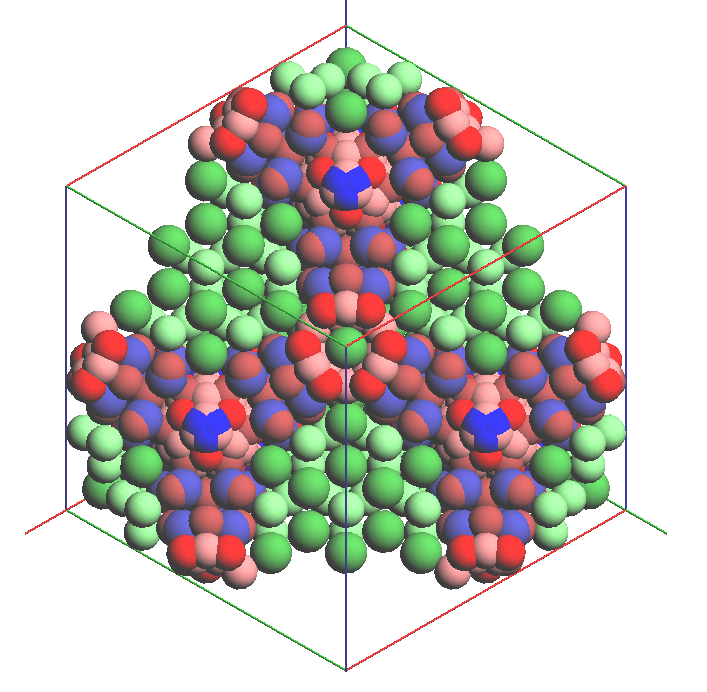
\includegraphics[scale=0.7]{rzut2}
	\caption{Przekr�j kom�rki elementarnej $\beta$- Mg$_{2}$Al$_{3}$.P�aszczyzna prostopad�a do kierunku [1,1,1].}
	\label{fig:rzut2}
\end{figure}

W temperaturze poni�ej 100\degree C stop $\beta$- Mg$_{2}$Al$_{3}$ wyst�puje w stanie fazy metastabilnej.
W temperaturze pomi�dzy 100 a 200\degree C zachodzi cz�ciowa transformacja do fazy $\beta\prime$, natomiast powy�ej 214\degree C faza $\beta\prime$ znika i zaobserwowa� mo�na tylko faz� $\beta$ (rysunek \ref{fig:diagram}\cite{Feuerbacher}. W kom�rce elementarnej stopu pozycje atomowe s� okre�lanie przez 23 krystalograficznie nier�wnowa�ne pozycje Wyckoffa\cite{PhysRev}. Generuje to w sumie 1832 mo�liwe do obsadzenia pozycje atomowe w kom�rce elementarnej, z kt�rych 840 jest obsadzonych z prawdopodobie�stwem r�wnym 1 przez atomy magnezu lub aluminium, natomiast prawdopodobie�stwo obsadzenia pozosta�ych atom�w jest mniejsze od 1. Dla pozycji, kt�rych prawdopodobie�stwo wynosi 1 istnieje lokalne ograniczenie odleg�o�ciowe r�wne 0,25092nm. Pozosta�e pozycje nie spe�niaj� tego ograniczenia. Pozycje o prawdopodobie�stwie r�wnym 1 uk�adaj� si� w szereg warstw heksagonalnych, prostopad�ych do kierunku [1,1,1] (g��wna przek�tna), tworz�c szkielet dla pozycji z du�ym udzia�em wakancji\cite{PhysRev}. 
%Pozycje z prawdopodobie�stwem r�wnym 1 tworz� szereg heksagonalny, kt�ry formuje szkielet dla pozycji o mniejszym prawdopodobie�stwie\cite{Wolny}.

\begin{figure}[h!]
  \centering
	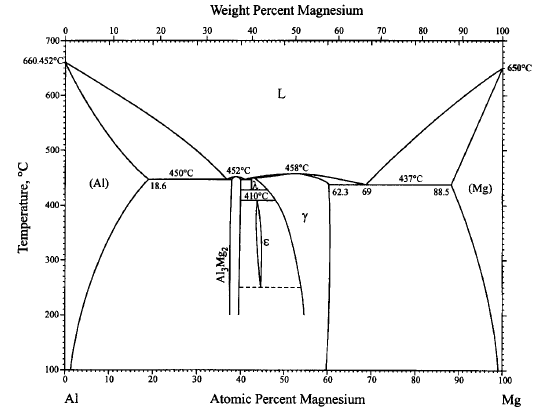
\includegraphics[scale=0.8]{diagram}
	\caption{Diagram fazowy stopu $\beta$- Mg$_{2}$Al$_{3}$.}
	\label{fig:diagram}
\end{figure}



%---------------------------------------------------------------------------

\section{Symulacje dyfuzji i porz�dkowania w CMA}
\label{sec:symulacje}

%Symulacje dyfuzji i porz�dkowania w CMA korzystaj� z kilku algorytm�w. Pierwszy z nich to metoda ,,dziel i rz�d�''. Metoda dziel i rz�d� s�u�y do projektowana algorytm�w, cz�sto rekurencyjnych. Skomplikowany problem dzielimy na mniejsze problemy, do momentu a� rozwi�zanie jest bezpo�rednie. Przyk�adami takiego podej�cia s� algorytmy quicksort, merge sort, szybka transformata Fouriera czy algorytm Euklidesa najwi�kszego wsp�lnego dzielnika - jeden z pierwszych algorytm�w typu ,,dziel i rz�d�'' \cite{cormen}. Problematyczne mo�e by� dodatkowe zu�ycie pami�ci, jakie wyst�puje przy algorytmach rekurencyjnych. Wi��e si� to z wykorzystaniem stosu wywo�a� funkcji. Oczywi�cie praktycznie ka�dy algorytm rekurencyjny da si� przekszta�ci� na algorytm iteracyjny, jednak zu�ycie pami�ci pozostaje bez zmian. W przypadku symulacji wszystkie pozycje zosta�y podzielone na mniejsze, sk�adaj�ce si� z 72 pozycji atomowych.

Pliki wynikowe chmc, wykorzystywane w niniejszej wizualizacji, s� plikami wyj�ciowymi symulacji, realizuj�cej metod� Monte Carlo z zamian� obsadze� pozycji przez dany typ atomu lub wakancj� nazywan� cz�sto symulacj� gazu sieciowego (Lattice Gas). Metoda wykorzystuje losow� zamian� obsadzenia pozycji z cz�ciow� akceptacj� wyniku takiej zamiany, co prowadzi do znalezienia rozk�adu optymalnego w danej temperaturze. Jest to najprostsza z mo�liwych symulacji, w kt�rej nie pozwalamy na zmian� po�o�e� przestrzennych pozycji krystalicznych, bior�c pod uwag� tylko zmienno�� obsadze� tych pozycji (przez atomy Mg, Al lub wakacje). W tym przypadku liczymy  energi� dla ka�dego kroku. Je�eli energia w nast�pnym kroku maleje, to akceptujemy zmian�, je�eli energia ro�nie, to akceptujemy zmian� z prawdopodobie�stwem proporcjonalnym do wzoru \ref{eq:prob}\cite{cormen}.

\begin{equation} \label{eq:prob}
 P(akc.) = e^{\frac{-\Delta E}{kT}}
\end{equation}
gdzie $\Delta E$ jest przyrostem energii, k sta�� Boltzmanna, a T oznacza temperatur�. %Krokiem MC jest zmiana dw�ch obiekt�w(atom lub wakancja) mi�dzy dwoma z ustalonych pozycji.

Energia jest wyznaczana z potencja��w z odpowiednim u�rednieniem oblicze� kwantowych (potencja� dwuatomowy). Oddzia�ywania mi�dzy elementami uk�adu s� opisywane wzorem \ref{eq:ene}.
\begin{equation} \label{eq:ene}
E = \sum_{i,j=1, j>1}^{N} U(r_{ij})
\end{equation}

gdzie $r_{ij} = | \vec{r_{i}} - \vec{r_{j}} |$ a $ U(r_{ij}) $ jest energi� potencjaln� w po�o�eniach $r_{i}$ oraz $r_{j}$\cite{simulation}.\\

Kolejnym algorytmem u�ywanym w symulacji jest symulowane wy�arzanie. Algorytm ten jest algorytmem heurystycznym, kt�ry pr�buje znale�� optymalne rozwi�zanie, przeszukuj�c przestrze� alternatywnych rozwi�za� problemu. Algorytm jest bardzo skuteczny, gdy chcemy ustali� najlepsze ekstremum po�r�d ekstrem�w lokalnych. Algorytm przypomina proces wy�arzania w metalurgii - st�d nazwa. Mo�na go z powodzeniem stosowa� do ca�ej gamy problem�w, jak cho�by problem komiwoja�era. Jest to przyk�ad algorytmu zach�annego\cite{sa}. W tym przypadku modyfikujemy nie tylko obsadzenie, ale r�wnie� pozycje (przesuni�cia). Daje to du�o wi�ksz� elastyczno�� i szybsz� ewolucj� systemu. Szukanie najni�szej energii odbywa si� przez wygrzewanie uk�adu w coraz ni�szej temperaturze. 

%Symulowane wy�arzanie jest wykorzystywane w ko�cowym etapie symulacji do optymalizacji pozycji atom�w.

Nast�pny algorytm, jaki jest wykorzystywany w symulacji, to dynamika molekularna(MD). Jest to numeryczne rozwi�zywanie i komputerowa symulacja przestrzeni fazowej dla zdefiniowanego modelu uk�adu moleku�. Stosuje si� metody numeryczne, poniewa� analityczne rozwi�zanie by�oby zbyt skomplikowane. Elementarnie stosuje si� r�wnania ruchu Newtona, kt�re wzbogaca si� o oddzia�ywania w celu uzyskania informacji o w�a�ciwo�ciach zale�nych od czasu. Oddzia�ywania mi�dzy elementami uk�adu s� opisywane przez funkcj� oraz zesp� parametr�w dla tej funkcji. Dynamika molekularna znajduje wiele zastosowa�, mi�dzy innymi w biochemii jako narz�dzie do poznawania struktury i oddzia�ywa� w bia�kach, kwasach nukleinowych i innych biomoleku�ach\cite{MD}. Temperatura jest kontrolowana przez ca�kowit� energi� kinetyczn� systemu.

Wyniki symulacji, zawarte w zbiorach ,,chmc'', kt�re stanowi� dane wej�ciowe dla konstruowanej aplikacji, pochodz� z symulacji, kt�ra operuje tylko obsadzeniami pozycji krystalicznych przez dwa typy atom�w (Mg, Al) lub wakancj�. W zbiorach tych zawarte s� u�rednione, po pewnych przedzia�ach czasu, prawdopodobie�stwa obsadze� odpowiednich pozycji krystalicznych oraz ich rozrzuty. Z punktu widzenia u�ytkownika wizualizacji wa�ne s� przede wszystkim prawdopodobie�stwa obsadze� oraz ich zmiany z czasem i temperatur�. Wizualizacja tych parametr�w mo�e da� istotne informacje o ewolucji systemu, np. o tym kt�re pozycje bior� g��wnie udzia� w procesach porz�dkowania, jakimi kana�ami zachodzi dyfuzja atom�w, w jakich temperaturach zachodz� poszczeg�lne typy proces�w porz�dkowania i do jakich struktur one prowadz�. U�wiadamiaj� one r�wnie� jaka jest skala czasowa proces�w porz�dkowania i jak d�ugo powinna by� prowadzona symulacja, aby uzyskane wyniki by�y miarodajne dla danych proces�w porz�dkowania. Jak wida� z powy�szego, aplikacja realizuj�ca wizualizacj� tych danych mo�e by� pomocna na wiele sposob�w osobom prowadz�cym badania nad tym procesami.


\chapter{Przegl�d potencjalnych technologii}
\label{cha:przegladTech}
W rozdziale opisz� technologie u�yte do stworzenia prototyp�w i finalnej aplikacji.

%---------------------------------------------------------------------------

\section{Zdefiniowanie wymaga� projektowych}
\label{sec:wymaganiaProjektowe}

Jednym z najwa�niejszych zada� podczas realizacji projektu jest zebranie i analiza wymaga� projektowych. Wymagania projektowe to zbi�r potrzeb danego produktu lub us�ugi, a tak�e spos�b ich dzia�ania. W in�ynierii oprogramowania zbi�r wymaga� jest wykorzystywany w fazie projektowania nowego produktu. Wymagania pokazuj�, jakie elementy i funkcje s� niezb�dne w konkretnym przypadku. Istnieje bardzo du�o modeli opisuj�cy ten proces. Wi�kszo�� z nich jest standaryzowana przez organizacje ISO oraz IEC pod numerem 12207 Systems and software engineering\cite{IsoIec2008}.

Przez zebraniem wymaga� cz�sto wykonuje si� jeszcze jeden etap - studium wykonalno�ci, kt�re sk�ada si� z analizy rynku, analizy ekonomicznej, analizy strategicznej oraz analizy technicznej. W zale�no�ci od rozmiaru projektu samo zbieranie wymaga�, mo�e zosta� podzielony na etapy. Jest to bardzo cz�sta praktyka w projektach rz�dowych\cite{req}. Faz� wymaga� dzielimy na:

\begin{enumerate}%[1)]
\item gromadzenie wymaga�
\item analizowanie
\item specyfikowanie
\item zatwierdzenie
\end{enumerate}

Dobre wymagania projektowe charakteryzuje\cite{req}:
\begin{enumerate}%[1)]
\item Aktualno�� - wymaganie powinno pozosta� aktualne z up�ywem czasu.
\item Jednoznaczno�� - wymaganie powinno by� jasno sformu�owane, bez subiektywnych opinii. �argon techniczny i akronimy powinny by� zdefiniowane w dokumencie. 
\item Kompletno�� - wymaganie powinno by� zdefiniowane w jednym miejscu z kompletem niezb�dnych informacji.
\item Obowi�zkowo�� - ka�de niezb�dny wymaganie musi zosta� zdefiniowane. Brak wymagania oznacza wykluczenie z projektu.
\item Poprawno�� - wymaganie wype�nia wszystkie lub cz�� potrzeb biznesowych, kt�re s� jasno okre�lone.

\item Sp�jno�� - wymaganie odnosi si� do jednej i tylko jednej sprawy.
\item Wykonalno�� - wymaganie musi by� wykonalne w ramach ogranicze� projektowych.
\item Weryfikowalno�� - wymaganie powinno by� weryfikowalne empirycznie lub poprzez analiz�.
\item Zgodno�� - wymagania nie powinny by� sprzeczne ze sob�.
\end{enumerate}

Istnieje wiele r�nych cech, kt�re charakteryzuj� dobre wymagania, ale s� one specyficzne dla danej domeny technologicznej. Istnieje jeszcze jeden istotny podzia� wymaga�. Podzia� na trzy kategorie:
\begin{enumerate}%[1)]
\item Wymagania funkcjonalne - definiuj�, co ma realizowa� system np. system powinien generowa� raporty.
\item Wymagania niefunkcjonalne - s� to wymagania jako�ciowe. Opisuj� bezpiecze�stwo, wydajno�� itp.
\item Wymagania ogranicze� - okre�laj� granice rozwi�zania.
\end{enumerate}

Wszystkie wymagania powinny by� weryfikowalne, poza wymaganiami ogranicze� typu ,,system nie powinien''.


\subsection{Model Kaskadowy}
\label{subsec:modelKaskadowy}

Pierwsze wzmianki o wymaganiach projektowych pochodz� z lat sze��dziesi�tych ubieg�ego wieku.\cite{appliedSoftware} IBM by� pionierem bada� dotycz�cych procesu tworzenia oprogramowania. W 1956 roku jeden z pracownik�w IBMu, Herbert D. Benington, podczas konferencji na temat zaawansowanych metod tworzenia oprogramowania, opisa� model kaskadowy (inaczej zwany wodospadowym)\cite{advencedSoft}.

Model kaskadowy podzielony jest na 7 chronologicznych cz�ci:\cite{waterfallModel}

\begin{enumerate}%[1)]
\item Tworzenie wymaga� projektowych
\item Projektowanie
\item Implementacja
\item Integracja
\item Testowanie i debugowanie
\item Wdra�anie
\item Utrzymanie i konserwacja
\end{enumerate}

Model kaskadowy jest sekwencyjny. G��wn� jego cech� jest podzia� na niezale�ne cz�ci, z kt�rych ka�da wykonywana jest po zako�czeniu poprzedzaj�cej. Zalet� takiego podej�cia jest wykrywanie b��d�w we wczesnych etapach. 
B��d wykryty podczas projektowania stanowi du�o mniejsze wyzwanie i jest �atwiejszy w naprawie, ni� defekt, kt�rego istnienie spostrze�ono dopiero w fazie wdra�ania. Jednak takie rozwi�zanie ma r�wnie� swoje wady. Najistotniejszym problemem jest brak mo�liwo�ci szybkiej zmiany na p�nym etapie projektu. W realnych warunkach wymagania zmieniaj� si� bardzo cz�sto, co dla nietrywialnych projekt�w mo�e oznacza� ci�g�e powroty do fazy projektowej. Bardziej fatalne w skutkach mo�e okaza� si� z�e okre�lenie wymaga� projektowych. Przyk�adowo:  podczas wdra�ania klient stwierdzi, �e oprogramowanie nie jest dostatecznie szybkie, co mo�e by� skutkiem ogranicze� technologicznych. W takim wypadku projekt jest zamykany. Kolejnym problemem jest s�abe wykorzystanie zasob�w ludzkich - testerzy musz� czeka� na zako�czenie pracy przez programist�w. W 2001 roku przeprowadzono badanie 1027 projekt�w IT w Wielkiej Brytanii. Okaza�o si�, �e techniki zarz�dzania narzucaj�ce metodologi� kaskadow� by�y jednym z najwi�kszych czynnik�w, kt�re wp�yn�y na pora�k� projektu \cite{sofscal}. Problemy te okaza�y si� na tyle powa�ne, �e dzisiaj nikt ju� nie korzysta z modelu kaskadowego. W genialny spos�b Edward V. Berard podsumowa� kompleksowe specyfikacje modelu kaskadowego.
\begin{quote}
Walking on water and developing software from a specification are easy if both are frozen.
\end{quote}
%\quote{}

%\newpage

\begin{figure}[h!]
  \centering
	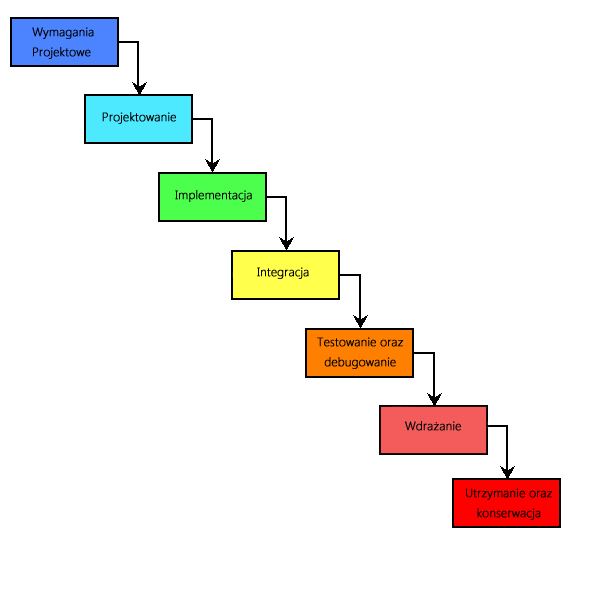
\includegraphics[scale=0.6]{waterfall}
	\caption{Schemat modelu kaskadowego.}
\end{figure}

\newpage

\subsection{Model spiralny}
\label{subsec:modelSpi}

Model spiralny jest to rodzaj procesu tworzenia oprogramowania. Kolejne etapy s� podzielone na mniejsze cz�ci. Ka�da z tych cz�ci jest cyklicznie powtarzana w p�tli, przez co plan jest przedstawiany w postaci spirali. Model spiralny, podobnie jak kaskadowy, posiada �cis�� kontrole nad projektem. W pocz�tkowej fazie ��czymy projektowanie z tworzeniem prototyp�w \cite{spiral}.

P�tle spirali s� podzielone na sektory:  
\begin{enumerate}%[1)]
\item Definicja cel�w
\item Rozpoznanie i redukcja zagro�e�
\item Implementacja i zatwierdzanie
\item Ocena i planowanie
\end{enumerate} 

Wyra�n� zalet� modelu spiralnego jest szczeg�owa analiza zagro�e�. Model spiralny, nie precyzuje w jaki spos�b maja by� realizowane poszczeg�lne p�tle np. mo�na u�y� modelu kaskadowego. Podobnie jak w modelu kaskadowym, usuwanie b��d�w w ko�cowych etapach jest bardzo kosztowne.

\begin{center}
	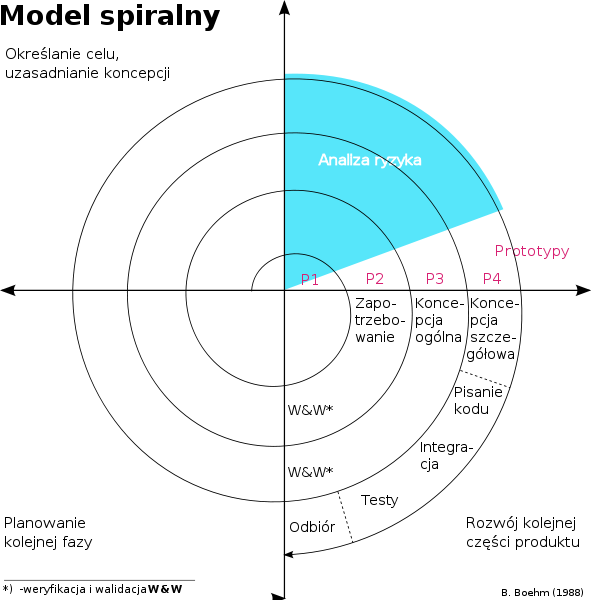
\includegraphics[scale=0.6]{ModelSpiralny}
	\captionof{figure}{Schemat modelu spiralnego. �r�d�o:\cite{spiral}. }
\end{center}

\subsection{Model iteracyjny}
\label{subsec:modelIter}

W odpowiedzi na wady modelu kaskadowego powsta�y modele iteracyjne. Pierwszy system wykonany w oparciu o model iteracyjny datuje si� na rok 1960. Powsta� on w ramach projektu Mercury, kt�ry by� sponsorowany przez NASA\cite{iterBrief}. Podstawowym pomys�em, kt�ry definiuje model iteracyjny, jest budowanie systemu poprzez powtarzalne cykle (iteracje). Podej�cie to pozwala deweloperom wyci�gn�� wnioski z dotychczasowej pracy, zwi�ksza elastyczno�� wymaga� w p�niejszym okresie oraz pozwala lepiej wykorzysta� zasoby firmy. Model iteracyjny jest cz�sto stosowany w wypadku, gdy pe�na funkcjonalno�� systemu nie jest wymagana. Klient mo�e otrzyma� cz�ciowo dzia�aj�cy system, aby lepiej oceni� jego funkcjonalno��.

\begin{figure}[h!]
  \centering
	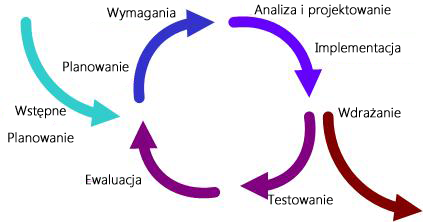
\includegraphics[scale=1.0]{itermodel}
	\caption{Schemat modelu iteracyjnego.}
\end{figure}

Oczywi�cie model iteracyjny posiada r�wnie� wady, takie jak dodatkowy koszt ka�dego cyklu czy trudno�� w podziale na iteracje. Pomimo tego, wszystkie wsp�czesne metody tworzenia oprogramowania bazuj� na idei iteracji.

Przyk�adem modelu iteracyjnego jest RUP (Rational Unified Process)\cite{rup}, kt�ry sk�ada si� z sze�ciu praktyk:

\begin{enumerate}%[1)]
\item Buduj iteracyjnie z ryzykiem jako najwa�niejszym czynnikiem
\item Zarz�dzaj wymaganiami
\item Wprowad� architektur� opart� na komponentach

\item Wprowad� modele wizualne oprogramowania
\item Ci�gle sprawdzaj jako��
\item Kontroluj zmiany
\end{enumerate} 

Pod koniec lat dziewi��dziesi�tych RUP dominowa� jako model budowania system�w zw�aszcza w �rodowiskach korporacyjnych i rz�dowych. Wad� tego rozwi�zania jest spora ilo�� dokumentacji - cz�sto wymagana np. przez regulatora - kt�ra wyd�u�a i usztywnia proces tworzenia systemu.

\subsection{Agile Manifesto}
\label{subsec:agileMan}

Jako reakcja na poziom komplikacji i koszty metod, takich jak kaskadowa, powsta�o wiele tzw. ,,lekkich'' metod. Oto niekt�re z nich:\cite{agileAndIter}

\begin{enumerate}%[1)]
\item Scrum (1995)
\item XP (Extreme Programming) (1996)
\item Crystal Clear

\item Feature Driven Development
\item Dynamic Systems Development Method (1995)
\end{enumerate} 

W 2001 roku fundacja non-profit Agile Alliance opublikowa�a ,,Agile Manifesto''. Manifest ten zawiera najwa�niejsze zasady nowo powsta�ych metodologii. Sk�ada si� on z 4 podpunkt�w:\cite{agileManifesto}

\begin{enumerate}%[1)]
\item Ludzie i interakcje ponad procesy i narz�dzia
\item Dzia�aj�ce oprogramowanie ponad wyczerpuj�c� dokumentacj�

\item Wsp�praca klienta ponad negocjacj� umowy
\item Reakcja na zmiany ponad wykonanie planu
\end{enumerate}

Metodologie Agile posiadaj� bardzo �cis�y opis procesu, dlatego zarz�dzanie projektem wymaga dyscypliny. Inspekcje wymaga� s� bardzo cz�ste, przez co szybko tworzone jest oprogramowanie wysokiej jako�ci. Agile kierowany jest g�ownie do ma�ych i �rednich zespo��w, dlatego dokumentacja jest ograniczona do minimum. Zespo�y programist�w Agile s� zazwyczaj wielofunkcyjne i samozarz�dzalne, z bardzo p�ask� hierarchi�. Bardzo du�y nacisk k�adzie si� na komunikacj� bezpo�redni�, dlatego bardzo popularne s� codzienne kilkunastominutowe spotkania.

Metody Agile dziel� zadania na ma�e procesy iteracyjne, kt�re nie zawieraj� planowania d�ugoterminowego. Iteracje s� kr�tkie. Trwaj� zazwyczaj od 1 do 4 tygodni. Ka�da iteracja zawiera pe�en proces: planowanie, analiza wymaga�, projektowanie, implementacja i testowanie. Na ko�cu dzia�aj�cy produkt jest przedstawiany klientom. Minimalizuje to ryzyko drastycznych zmian w wymaganiach projektu. Bardzo cz�sto, aby zminimalizowa� komunikacj�, przedstawiciel klient�w jest cz�onkiem zespo�u.\cite{agileManifesto}.

\subsection{The Lean Startup}
\label{subsec:lean}

Bardzo ciekawe podej�cie opisuje Eric Ries w swojej ksi��ce ,,The Lean Startup''. Opisuje on sytuacje, w kt�rych cz�sto nie mo�na stworzy� specyfikacji, poniewa� klient nie wie dok�adnie, jakiego produktu oczekuje lub jest to produkt innowacyjny. Filozofia ,,The Lean Startup'' opiera si� na procesie produkcji Lean Manufacturing. Jest to proces opracowany w japo�skich fabrykach samochod�w, kt�ry minimalizuje straty poprzez redukcj� koszt�w, kt�re nie tworz� warto�ci dla klienta. W szczeg�lno�ci system koncentruje si� na odpowiednim umieszczeniu ma�ych zapas�w niezb�dnych materia��w(zwanych Kanban) na ca�ej linii produkcyjnej, zamiast przechowywania zapas�w w magazynie centralnym. Zmniejsza to straty i zwi�ksza produktywno��, z drugiej strony trudniejsze staje si� zarz�dzanie zasobami(g��wnie surowcami i p�produktami) \cite{lean}.

Z filozofi� Lean Startup wi��e si� pi�� kluczowych poj��:
\begin{enumerate}%[1)]
\item Minimum viable product - jest to produkt, kt�ry pozwala nam na zebranie jak najwi�kszej liczby potwierdzonych fakt�w o klientach, przy jak najmniejszym koszcie. Pozwala rozpocz�� proces badania potrzeb klient�w jak najwcze�niej.
\item Continuous deployment - jest to proces, w kt�rym ka�dy nowy kod jest natychmiast wdra�any.
\item Split testing (inaczej zwany A/B test) - jest to rodzaj testu, w kt�rym tej samej grupie klient�w pokazujemy dwie lub wi�cej wersji danego produktu. Dzi�ki temu mo�emy wybra� wersj�, kt�ra odpowiada klientom bardziej oraz okre�li� kierunek rozwoju.
\item Vanity metrics - jest to rodzaj metryki, w jaki spos�b firmy pr�buj� okre�li� wzrost biznesu, tak aby by� on jak najlepszy. Cz�sto daje to fa�szywy obraz.
\item Pivot - jest to kontrolowana, gruntowna zmiana produktu lub strategii.
\end{enumerate}

Filozofia Lean Startup jest nie tylko z powodzeniem stosowana do produkt�w IT - korzystaj� z niej r�wnie� inne bran�e.

\section{Specyfikacja programu do wizualizacji CMA}
\label{subsec:specCMA}
Gdy zaczyna�em budowa� program do wizualizacji stop�w mi�dzymetalicznych, postanowi�em zebra� wymagania wed�ug danego planu:

\begin{enumerate}%[1)]
\item Wymaganie powinny by� podzielone na podpunkty
\item Ka�dy podpunkt powinien zawiera�, co jest wymagane - bez okre�lenia jak to zostanie zrobione
\item Ka�dy podpunkt powinien by� ,,atomowy''. Na przyk�ad ,,Program powinien wy�wietli� 1000 obiekt�w oraz tworzy� animacje 1000 obiekt�w'' nale�y rozbi� na 2 podpunkty ,,Program powinien wy�wietli� 1000 obiekt�w'' oraz ,,Program powinien tworzy� animacje 1000 obiekt�w''
\item Powinien by� jasno okre�lony cel, wymagania projektowe oraz specyfikacja funkcjonalna
\item Nale�y okre�li� wymagania bezpiecze�stwa

\item Wymagania niefunkcjonalne powinny okre�la� wydajno�� i dost�pno��
\item Nale�y okre�li� co nie jest wymagane tak aby odr�ni� elementy przypadkowo pomini�te
\item Nale�y okre�li� spos�b komunikacji z innymi komponentami lub systemami
\end{enumerate} 

Po kilku drobnych zmianach ostateczna wersja specyfikacji sk�ada�a si� z 13 podpunkt�w dla wymaga� projektowych i 11 podpunkt�w specyfikacji funkcjonalnej:

\textbf{Cel:}

Celem projektu jest stworzenie aplikacji do wizualizacji proces�w dyfuzji i porz�dkowania w stopach mi�dzymetalicznych. Aplikacja powinna korzysta� z graficznego interfejsu, tak aby narz�dzie do analizy by�o wygodne w u�yciu.

\textbf{Wymagania projektowe:}
\begin{enumerate}%[1)]
\item Program dzia�a pod systemem Windows (zalecany jest Windows 7 lub wy�szy, mo�liwe jest wspieranie innych system�w)
\item Program dzia�a pod kontrol� �rodowiska .Net
\item Program powinien obs�u�y� klika tysi�cy modeli 3D jednocze�nie, dzia�aj�c p�ynnie dla operacji, takich jak obr�t
\item Program powinien obs�ugiwa� r�ne rozdzielczo�ci ekran�w
\item Program powinien informowa� u�ytkownika o post�pie zada� trwaj�cych wi�cej ni� 5 sekund

\item Program powinien obs�ugiwa� pliki w formacie .chmc
\item Parametry modeli, taki jak kolor, prze�roczysto�� musz� by� zgodne z warto�ciami symulacji
\item Program powinien tworzy� rzuty modeli dla grupy plik�w wej�ciowych symulacji
\item Dla ka�dej klatki animacji musz� zosta� uwzgl�dnione parametry pocz�tkowe ustawione przez u�ytkownika
\item Program powinien zu�ywa� mniej ni� 1GB ramu dla liczby obiekt�w poni�ej 3000

\item Dost�pno�� programu jest wy��cznie zale�na od komputera, na kt�rym aplikacja si� znajduje
\item Program nie powinien ��czy� si� z us�ugami internetowymi lub sieciowymi
\item Program nie powinien ��czy� si� z innymi komponentami
\end{enumerate}

\newpage

\textbf{Specyfikacja funkcjonalna:}
\begin{enumerate}%[1)]
\item U�ytkownik mo�e otworzy� plik, aby wczyta� model
\item U�ytkownik mo�e obraca� modelem 3D 
\item U�ytkownik mo�e powi�kszy� model
\item U�ytkownik mo�e precyzyjnie wybra� skale modelu
\item U�ytkownik mo�e wr�ci� do parametr�w pocz�tkowych

\item U�ytkownik mo�e zmieni� parametry kamery
\item U�ytkownik mo�e skalowa� modele
\item U�ytkownik mo�e zapisa� zrzut ekranu na kt�rym znajduje si� model
\item U�ytkownik ma mo�liwo�� filtrowania modeli poprzez ustawienie maski
\item U�ytkownik mo�e przetwarza� grup� plik�w do stworzenia animacji

\item U�ytkownik mo�e zmieni� warto�� kana�u alfa modeli
\end{enumerate}  
Zaleta tak zwi�z�ej specyfikacji jest �atwo�� ewentualnych zmian oraz kr�tki czas nauki dla dewelopera.

%---------------------------------------------------------------------------

\section{Prototypy r�nych technologii}
\label{sec:prototypy}

Po zebraniu wszystkich wymaga� projektowych mog�em przyst�pi� do budowy kilku prototyp�w r�nych technologii, by sprawdzi�, kt�ra najlepiej spe�nia wymagania. Prototypownie jest o tyle istotne, �e daje nam empiryczny dow�d mo�liwo�ci danej technologii. Jako potencjalnych kandydat�w wytypowa�em cztery technologie, kt�re posiadaj� wsparcie dla grafiki 3D: 

\begin{enumerate}%[1)]
\item OpenGL
\item XNA
\item WPF
\item DirectX
\end{enumerate}  

OpenGL (ang. Open Graphics Library) - jest otwartym standardem API, s�u��cym do generowania grafiki. Biblioteka umo�liwia prace na najni�szym poziomie, w zwi�zku z tym bardzo cz�sto korzysta si� z rozszerze�, silnik�w lub framework�w. Filozofia dzia�ania OpenGL opiera si� na maszynie stanowej \cite{openGLspec}. Biblioteka ma dwa g��wne cele. Stworzy� jednolity interface niezale�ny od sprz�tu oraz wpiera� standard w pe�ni, nawet w przypadku braku funkcjonalno�ci w sprz�cie (emulacja oprogramowaniem). OpenGL jest bezpo�rednim konkurentem DirectX.

XNA - jest to framework do tworzenia gier w ramach platformy .Net. Pocz�tkowo powsta� on dla konsoli Xbox, ale zosta� rozszerzony na ca�y ekosystem Microsoftu. Dzia�a on na relatywnie niskim poziomie. Posiada wiele cech wsp�lnych z technologi� DirectX, takich jak wsparcie dla grafiki 3D, jednak kod jest w pe�ni zarz�dzany. Dost�pne jest r�wnie� opensoucowa implementacja Mono.XNA, kt�ra dzia�a na innych systemach, takich jak Mac OS X czy Linux. Pomimo i� XNA powsta�o jako framework do gier, z powodzeniem jest stosowany do innych zada�. Przyk�adowo XNA Math s�u�y do oblicze� matematycznych na jednostce graficznej\cite{xnaUrl}.

WPF (ang. Windows Presentation Foundation) - jest cz�ci� platformy .Net, s�u��c� do tworzenia aplikacji graficznych. Do definicji obiekt�w u�ywany jest XAML (pochodna XMLa), kt�ry zwi�ksza mo�liwo�ci budowania bogatych interfejs�w bez ingerencji programisty. Grafik, tworz�c interface graficzny, tworzy� tylko szablon dla programisty, kt�ry implementowa� wszystkie elementy. Korzystaj�c z XAML i narz�dzi, takich jak Blend, grafik jest w stanie stworzy� w pe�ni funkcjonalne GUI bez pomocy programisty. Po�rednio korzysta z DirectX, wy��cznie poprzez interface z kodu zarz�dzanego.\cite{wpf}.

DirectX jest kolekcj� API do tworzenia grafiki 2D i 3D. G��wnie wykorzystywana w grach i aplikacjach multimedialnych. DirectX jest technologi� Microsoftu, kt�ra wspiera r�wnie� efekty d�wi�kowe do gier, obs�ug� urz�dze� peryferyjnych itp. DirectX, poza wsparciem dla multimedi�w, oferuje r�wnie� DirectCompute. Technologia umo�liwia wykorzystanie DirectX do obs�ugi oblicze� GPGPU. Aby korzysta� bezpo�rednio z DriectX, nale�y aplikacje napisa� w j�zyku C lub C++\cite{directX}.

OpenGL i DirectX z pewno�ci� poradzi�by sobie z programem do wizualizacji w sensie wydajno�ciowym. Problemem staje si� tworzenie przycisk�w, suwak�w i innych kontrolek. Obie technologie pracuj� na bardzo niskim poziomie, dlatego wymagaj� sporych nak�ad�w pracy. W przypadku XNA i WPF nie mia�em do�wiadczenia, kt�re potwierdza�oby spe�nienie wymaga� projektowych, dlatego stworzy�em 2 prototypy.

\newpage

Pierwszy prototyp bazowa� na XNA. Po za�adowaniu testowych plik�w prototyp spe�ni� wszystkie wymagania stawiane w specyfikacji.

\begin{figure}[h!]
  \centering
	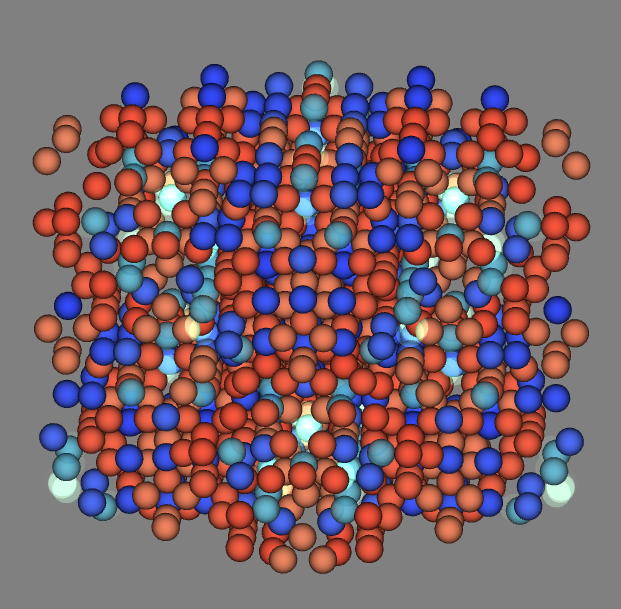
\includegraphics[scale=0.7]{xna1}
	\caption{Zrzut ekranu pierwszego prototypu (XNA).}
\end{figure}

Kolejny prototyp powsta� w WPF. Po za�adowaniu modeli dzia�a� on wyra�nie wolniej od pierwszego, jednak na tyle dobrze, �e spe�ni� wszystkie wymagania projektowe.


\begin{figure}[h!]
  \centering
	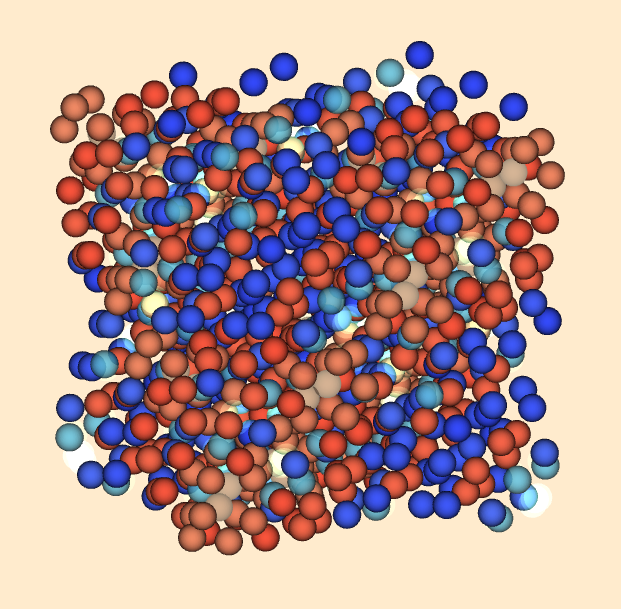
\includegraphics[scale=0.7]{wpf1}
	\caption{Zrzut ekranu drugiego prototypu (WPF).}
\end{figure}

Reasumuj�c, ka�da z wyszczeg�lnionych technologii spe�ni�a wszelkie kryteria, postanowi�em jednak wybra� WPF. Jest to technologia najbardziej optymalna pod wzgl�dem po�wi�conego czasu in�ynieryjnego. Posiada wbudowany uk�ad wsp�rz�dnych w trzech wymiarach, kamer�, predefiniowane tekstury i wiele innych. Integracja z graficznym interfejsem nie wymaga �adnej dodatkowej pracy w odr�nieniu od XNA. 




\chapter{Implementacja aplikacji}
\label{cha:implementacjaApp}
W rozdziale opisz� projekt aplikacji. Om�wi� struktur� programu, interefejs u�ytkownika, u�yte algorytmy oraz przedstawi�, jak aplikacja zosta�a przetestowana.

%---------------------------------------------------------------------------

\section{Struktura aplikacji}
\label{sec:strukturaApp}
Struktura omawianej aplikacji opiera si� na wzorcu architektonicznym Model View Controller (MVC). Wzorce architektoniczne okre�laj� sprawdzony spos�b tworzenia architektury systemu. Definiuj� one, z jakich element�w sk�ada si� system, og�lna struktur� komponent�w, komunikacj� pomi�dzy modu�ami oraz jaki zakres funkcjonalno�ci przypada na ka�dy komponent. 

MVC g��wnie u�ywany jest w aplikacjach, posiadaj�cych interfejs graficzny. Sk�ada si� on z 3 cz�ci:
\begin{enumerate}%[1)]
\item Model - okre�la logik� aplikacji
\item View - odpowiada za prezentowanie danych u�ytkownikowi
\item Kontroler - opisuje, jak Model komunikuje si� z View.
\end{enumerate}

Nieroz��cznymi elementami ka�dej aplikacji s� struktury danych, algorytmy i komunikacja. MVC silnie separuje ka�dy z element�w. Przyk�adowo, w dobrze zaprojektowanej aplikacji kod wy�wietlaj�cy informacje u�ytkownikowi nie mo�e znajdowa� si� w modelu. Do zalet tego wzorca nale��:
\begin{enumerate}%[1)]
\item Niezale�no�� modelu i widoku - mo�na zmieni� wygl�d lub doda� inny do aplikacji bez konieczno�ci ingerencji w model
\item Lepsza podatno�� na zmiany - zespo�y pracuj�ce nad widokiem i modelem mog� pracowa� niezale�nie
\end{enumerate}

Natomiast wady to:
\begin{enumerate}%[1)]
\item Z�o�ono�� - aplikacje oparte na tym wzorcu bywaj� rozbudowane, dlatego najcz�ciej stosuje si� go wobec �rednich i du�ych projekt�w
\item Kosztowne zmiany interfejs�w 
\end{enumerate}

MVC jest bardzo popularnym wzorcem po�r�d aplikacji internetowych, gdzie widok jest definiowany w j�zyku HTML, model okre�la aplikacja serwerowa i komunikacja na og�l opiera si� na ��daniach HTTP\cite{fowler}. Windows Presentation Foundation opiera si� na wzorcu MVVM (Model View  View-Model), jednak nie korzysta�em z niego w swojej aplikacji - cechy jakie posiada MVVM nie by�y konieczne. Struktur� widoku wizualizacji najlepiej oddaje rysunek ~\ref{fig:guistruc}.

\begin{figure}[h!]
  \centering
	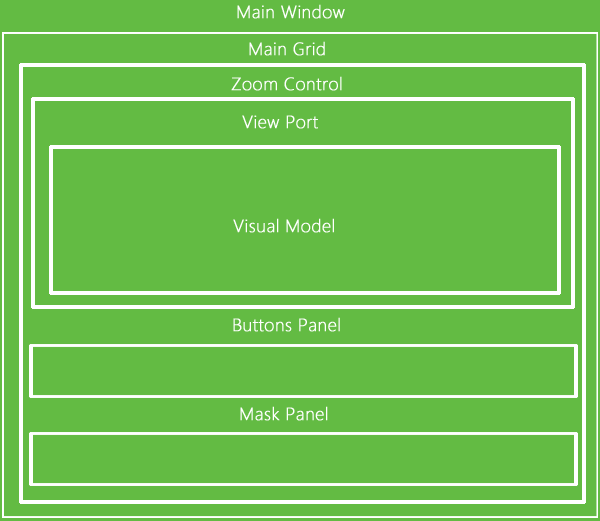
\includegraphics[scale=0.7]{guistruc}
	\caption{Struktura widoku - podzia� na kontenery.}
	\label{fig:guistruc}
\end{figure}

W g��wnym oknie osadzony jest kontener typu Grid (Main Grid). Jest to rodzaj panelu, kt�ry pozwala na umieszczenie wielu element�w wewn�trz. Zoom Control s�u�y do powi�kszania i pomniejszania modeli. Obok niego jest panel, w kt�rym znajduj� si� guziki oraz suwaki (Buttons Panel) i panel z filtrem maski (Mask Panel). Najistotniejszy, z punktu widzenia u�ytkownika, jest panel typu Viewport3D (View Port), kt�ry odpowiada ze wy�wietlanie obiekt�w w trzech wymiarach. W �rodku znajduje si� Visual Model, do kt�rego przypisany jest model atom�w\cite{wpf}. Dzi�ki takiej strukturze aplikacja w �atwy spos�b dostosowuje si� do r�nych rozdzielczo�ci ekranu.

W aplikacji mo�na wyszczeg�lni� kilka wzorc�w projektowych, kt�re s� wszechobecne w�r�d program�w. Deweloperzy bardzo cz�sto korzystaj� z wzorc�w, cz�sto niejawnie, aby wykorzysta� najlepsze i sprawdzone rozwi�zanie. Jednym z wzorc�w kreacyjnych, z kt�rych korzystam jest Budowniczy. Dzi�ki niemu mo�na oddzieli� tworzenie obiekt�w od logiki, co pozwala nam u�ywa� tego samo procesu dla r�nych obiekt�w np. obiekt�w s�u��cych do test�w\cite{builder}. Na podstawie plik�w wynikowych i parametr�w ustawionych przez u�ytkownika program tworzy modele atom�w w kom�rce elementarnej. U�ywana do tego jest klasa AtomBuilder, kt�ra z kolekcji atom�w tworzy model 3D.

Program do wizualizacji sk�ada si� z 5569 niepustych linii kodu, 11 plik�w i biblioteki WPFExtenstion, kt�ra nie wchodzi w sk�ad standardowej biblioteki. Rysunek ~\ref{fig:solution} przedstawia struktur� projektu:

\begin{figure}[h!]
  \centering
	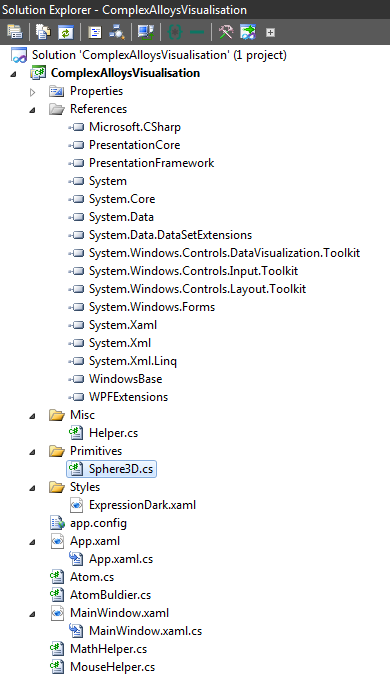
\includegraphics[scale=0.6]{solution}
	\caption{Struktura projektu Complex Alloys Visualisation.}
		\label{fig:solution}
\end{figure}

Properties zawieraj� informacje, takie jak numer identyfikacyjny biblioteki lub pliku wykonywalnego. Folder References okre�la wszystkie zale�no�ci, jakie posiada projekt. W folderze Misc znajduje si� klasa Helper, definiuj�ca metody pomocnicze. Nast�pnie folder Primitives posiada klas� Sphere3D, kt�ra definiuje teselacje sfery. Plik ExpressionDark.xaml w folderze Styles okre�la wygl�d GUI. App.xaml oraz App.xaml.cs okre�laj� punkt startowy aplikacji oraz obiekty istniej�ce przez ca�y czas istnienia procesu. Klasa Atom definiuje obiekt reprezentuj�cy pojedynczy atom. AtomBuilder tworzy model z atom�w. MainWindow.xaml odpowiada z GUI w oknie g��wnym. MainWindows.xaml.cs okre�la interakcje u�ytkownika z programem. MathHelper posiada funkcj� do konwersji stopni na radiany. Klasa MouseHelper okre�la w jaki spos�b myszka mo�e obraca� model.  

%---------------------------------------------------------------------------

\section{U�yte Algorytmy i Struktury Danych}
\label{sec:uzyteAlgo}

Aplikacja w pe�ni napisana jest w j�zyku obiektowym C\#. W ksi��ce ,,J�zyk C\# Programowanie'' znalaz�em bardzo dobr� definicj� j�zyka:
\begin{quote}
C\# (wymawiane jako ,,si szarp'' to prosty, nowoczesny, obiektowy i bezpieczny pod wzgl�dem stosowania typ�w j�zyk programowania. Korzenie C\# tkwi� w rodzinie j�zyk�w C, dzi�ki czemu szybko b�d� go mogli przyswoi� programi�ci u�ywaj�cy C, C++ i Java. Standaryzacj� C\# zajmuje si� organizacja ECMA International, kt�ra opracowa�a norm�  ECMA-334, oraz IOS/IEC, odpowiedzialna za norm� ISO/IEC 23270. Kompilator j�zyka C\# oferowany przez firm� Microsoft w ramach platformy .Net spe�nia wymogi obydwu wymienionych standard�w. 

C\# jest j�zykiem obiektowym, lecz zapewnia tak�e wsparcie dla programowania komponentowego (ang. component-oriented). Nowoczesne sposoby projektowania oprogramowania w coraz wi�kszym stopniu opieraj� si� na komponentach programowych, maj�cych posta� niezale�nych i samoopisuj�cych si� pakiet�w funkcji. Kluczem do tego typu komponent�w jest to, �e prezentuj� one model programowania za pomoc� w�a�ciwo�ci, metod i zdarze�, s� wyposa�one w atrybuty udost�pniaj�ce deklaratywne informacje na temat komponentu, a tak�e zawieraj� swoj� w�asn� dokumentacj�. C\# umo�liwia korzystanie z konstrukcji j�zykowych, kt�re w bezpo�redni spos�b wspieraj� wymienione koncepcje, co czyni go niejako naturalnym j�zykiem do tworzenia i u�ywania komponent�w programowych\cite{csharp}.
\end{quote}

J�zyk ten jest kompilowany do kodu po�redniego Common Intermediate Language (CIL), kt�ry jest wykonywany przez �rodowisko uruchomieniowe. Natywnie wspieranym �rodowiskiem jest .Net dzia�aj�cy pod system Windows. Istnieje r�wnie� alternatywna, otwarta implementacja Mono, kt�ra wspiera wiele system�w operacyjnych. J�zyk C\# jest stosunkowo m�odym j�zykiem. Pierwsza wersja powsta�a w 2001 roku. C\# posiada bardzo wiele przydatnych cech, takich jak zarz�dzanie pami�ci�, wyra�enia LINQ czy pe�na kontrola typ�w. Jednak dla mnie najbardziej u�yteczna jest wieloparadygmowo�� j�zyka. C\# w wersji 1.0 pozwala� na pisanie kodu obiektowego oraz proceduralnego. C\# 2.0 doda� wsparcie dla programowania generycznego. C\# 3.0 zosta� wzbogacony o elementy programowania funkcjonalnego poprzez wyra�enia lambda oraz LINQ. C\# 4.0 doda� wsparcie dla programowania dynamicznego, natomiast C\# 5.0 wspiera programowanie asynchroniczne. Na dan� chwil� nie istnieje �aden inny mainstreamowy j�zyk, kt�ry wspiera�by tak wiele metodologii programowania. J�zyk ten posiada r�wnie� ma�o tzw. ,,gotcha'' (sprzeczne z intuicj� rozwi�zanie, kt�re powoduje b��dy w programowaniu), przez co programy zawieraj� mniej b��d�w. Moim zdaniem jest to istotna cecha, kt�ra wp�ywa na jako�� oprogramowania. Ludzki m�zg posiada swoje ograniczenia, wi�c korzystaj�c z prostszych narz�dzi, mo�emy budowa� bardziej skompilowane systemy\cite{csharp}.

\subsection{Funkcje pomocnicze}
\label{subsec:funkcjePom}

Ka�da aplikacja �redniej lub du�ej wielko�ci posiada zbi�r funkcji pomocniczych. Pomagaj� one w ograniczeniu powtarzaj�cego si� kodu w obr�bie programu. Dlaczego tworzy� zbi�r funkcji zamiast biblioteki? Poniewa� cz�sto s� zbyt specyficzne dla danej domeny problemu, aby z�o�y� z nich bibliotek�. Programista ma zawsze mo�liwo�� wniesienia zmian wed�ug wymaga�. Na potrzeby aplikacji stworzy�em 3 funkcje pomocnicze. Pierwsza z nich s�u�y do zamiany stopni na radiany wed�ug powszechnie znanego wzoru:

\begin{equation}
 \frac{stopnie}{180} * \Pi
\end{equation}

Dwie kolejne metody s�u�� do parsowania �a�cuch�w tekstowych i zamiany na liczb� zmiennoprzecinkow�. Dlaczego definiowa� na nowo tak prost� funkcj�, kt�ra istnieje w wielu bibliotekach? S� ku temu dwa powody: r�ny separator dziesi�tny oraz formatowanie liczb.

\begin{figure}[h!]
  \centering
	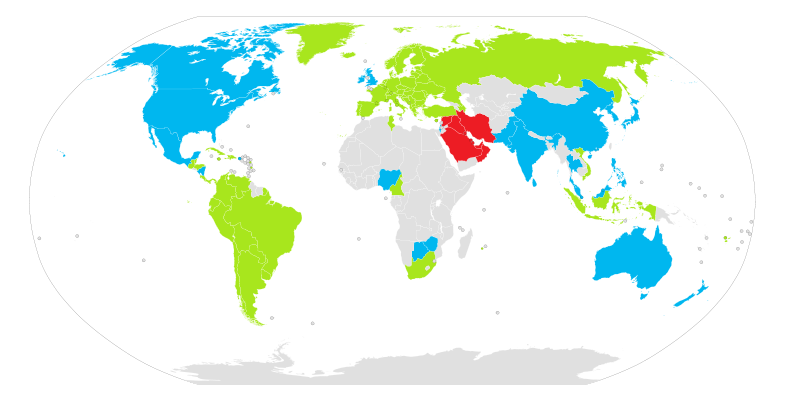
\includegraphics[scale=0.6]{separator}
	\caption{Rodzaje separator�w dziesi�tnych na �wiecie. Zielony: przecinek. Niebieski: kropka. Czerwony: momayyez.
	 �r�d�o: Wikipedia na licencji Creative Commons.}
\end{figure}

Na �wiecie dominuj� dwa r�ne separatory. Pierwszy z nich to kropka, kt�ry na powy�szej mapce zaznaczony jest kolorem niebieskim. Drugi to przecinek - kolor zielony. Istnieje r�wnie� trzeci separator, momayyez, kt�ry wyst�puje w krajach arabskich. U�ycie nieprawid�owego separatora dziesi�tnego mo�e mie� r�ne rezultaty. Najmniej szkodliwe jest oczywi�cie nieprawid�owe wy�wietlanie, natomiast bardzo cz�sto aplikacja zmienia swoje dzia�anie lub zawiesza si�. Fakt ten wynika z niewiedzy, ignorancji lub b��du w projekcie, tak jak w przypadku platformy .Net. Domy�lnie ustawiony jest lokalny separator, dlatego przyk�adowo aplikacja czytaj�ca plik w Wielkiej Brytanii mo�e dzia�a� poprawnie, natomiast w Polsce zawiesza si�. Jest kilka rozwi�za� dla tego problemu. Je�eli posiadamy �r�d�a programu, mo�emy poprawi� kod, kt�ry sprawia problemy. W przypadku braku dost�pu do kodu �r�d�owego mo�emy stworzy� modu�, kt�ry b�dzie konwertowa� pliki. Innym sposobem jest zmiana ustawie� u�ytkownika, jednak  mo�e to wp�yn�� na inne aplikacje. Najlepszym rozwi�zaniem jest stworzenie nowego u�ytkownika z odpowiednimi ustawieniami tylko dla tej aplikacji.

Aby unikn�� tego b��du, moja funkcja korzysta z wbudowanej funkcji z odpowiednimi parametrami:

\begin{lstlisting}
static bool TryParseDouble(this string text, out double value)
{
   return double.TryParse(text, NumberStyles.Any,
    CultureInfo.InvariantCulture, out value);
}
\end{lstlisting}

Funkcja akceptuje ka�dy format liczby zmiennoprzecinkowej. Dobr� praktyk� jest akceptowanie wi�kszego zbioru danych, aby p�niej odpowiednio je filtrowa�. Zdefiniowana metoda jest metod� rozszerze�. Mo�na j� rozpozna� po s�owie kluczowym ,,this''. Dzi�ki temu mo�na j� u�y�, jakby by�a zdefiniowana w typie string. Druga metoda ma to samo zadanie, jednak dodatkowo wy�wietla b��d dla u�ytkownika w postaci czerwonego tekstu. �wiadczy on o nieprawid�owym formacie liczby.

\begin{figure}[h!]
  \centering
	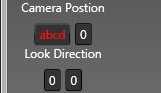
\includegraphics[scale=1.0]{abcd}
	\caption{Nieprawid�owa pozycja kamery.}
\end{figure}

\subsection{Klasa Sphere3D}
\label{subsec:sphere}

Model ka�dego atomu jest przedstawiany jako sfera. Kszta�t pojedynczej sfery jest tworzony w kodzie przy pomocy algorytmu teselacji, kt�ry definiuje poni�szy pseudokod:

\begin{enumerate}%[1)]
\item Ustalamy warunki pocz�tkowe: powierzchnia sfery sk�ada si� z 32 tr�jk�t�w
\item Budujemy sfer�, pos�uguj�c si� k�tem theta z zakresu <0; 360> oraz zmienn� y z zakresu <-1;1>
\item Tworzymy pusta siatk� MeshGeometry3D
\item Dla krok�w dt oraz dy dodajemy do siatki pozycje punkt�w, normalne oraz wsp�rz�dne tekstury 
\item ��czymy punkty tr�jk�tami
\item ,,zamra�amy'' siatk� 
\end{enumerate}

Tak stworzona siatka mo�e zosta� wykorzystana wielokrotnie, dlatego obliczana jest tylko raz.

\subsection{Klasa Atom}
\label{subsec:atom}

Klasa atom definiuje struktur� danych dla pojedynczego atomu. Seria atom�w jest tworzona podczas parsowania pliku z parametrami. Ka�dy atom ma nast�puj�ce parametry:
\begin{enumerate}%[1)]
\item Wsp�rz�dne x, y oraz z wyra�one jako wzgl�dna warto�� z zakresu <-0,5; 0,5> 
\item D�ugo�� kom�rki elementarnej
\item Rodzaj atomu (Magnez lub Aluminium)
\item Prawdopodobie�stwo wyst�pienia wakancji
\item Prawdopodobie�stwo obsadzenia atomem Aluminium
\item Prawdopodobie�stwo obsadzenia atomem Magnezu 
\item Sta�a konwersji do Angstrem�w (28,289)
\end{enumerate}

Dzi�ki tym parametrom mo�emy zbudowa� model siatki krystalicznej dla kom�rki elementarnej.

\subsection{Klasa AtomBuilder}
\label{subsec:atomBuilder}

Metoda CreateModel w klasie AtomBuilder tworzy model 3D na podstawie kolekcji atom�w. Podczas implementacji algorytmu napotka�em pierwsze ograniczenie narzucone przez WPF. Jest to brak bezpo�redniego dost�pu do Z-buffer, kt�ry odpowiada za zarz�dzanie g��bi� w przestrzeni tr�jwymiarowej. Dzi�ki Z-bufferowi rysowane s� tylko te elementy, kt�re s� widoczne. Problem pojawia si�, gdy niekt�re elementy s� ca�kowicie lub cz�ciowo prze�roczyste. Domy�lnie tekstura DiffuseMaterial u�ywa Z-buffer, przez co prze�roczyste atomy na pierwszym planie zas�aniaj� te na dalszym\cite{wpf}.

\begin{figure}[h!]
  \centering
	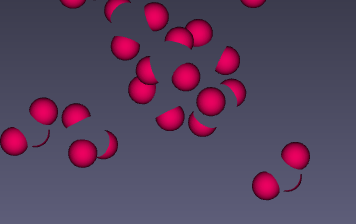
\includegraphics[scale=1.0]{zbuffer}
	\caption{Materia� u�ywaj�cy Z-buffer.}
\end{figure}

Jako rozwi�zanie tego problemu doda�em drobn� modyfikacj�. Je�eli prze�roczysto�� atomu jest poni�ej 30\%, zmieniam materia� na EmissiveMaterial, kt�ry nie zapisuje warto�ci do Z-buffera.

Podczas wizualizacji modeli kolor jest jednym z kluczowych parametr�w. Dostarcza u�ytkownikowi informacje o prawdopodobie�stwie obsadzenia. Zale�no�ci pomi�dzy kolorem a prawdopodobie�stwem opisuje dana tabelka:
\begin{table}
\begin{center}
    \begin{tabular}{ | l | p{3cm} | p{3cm} | p{3cm} | p{3.5cm} |} %p{4cm} 
    \hline
    Kana� Alfa & Prawd. wakancji & Prawd. Obsadzenia Mg & Prawd. Obsadzenia Al & Komentarz \\ \hline
    0 & 1 & 0 & 0 & Brak atomu \\ \hline
    1 & 0 & 1 & 0 & Atom Mg (kolor niebieski) \\ \hline
    1 & 0 & 0 & 1 & Atom Al (kolor czerwony) \\ \hline
    0,5 & 0,5 & 0,5 & 0 & Mg 50\%  \\ \hline
    0,5 & 0,5 & 0 & 0,5 & Al 50\% \\ \hline
    1 & 0 & 0,5 & 0,5 & Jest pe�ne obsadzenie, ale mieszane \\ \hline
    \hline
    \end{tabular}
    \caption{Zale�no�� prawdopodobie�stwa i koloru.}
\end{center}
\end{table}

Sumaryczne prawdopodobie�stwo ka�dej ze sk�adowych wynosi 1. Wszystkie warto�ci po�rednie powstaj� przez mieszanie si� barwy czerwonej i niebieskiej. Niestety kolor sk�adaj�cy si�  z 50\% czerwonego oraz 50\% niebieskiego nie jest zbyt wyra�ny. Dlatego aby polepszy� kontrast i jako�� modelu, dodatkowo wyst�puje kana� zielony. Ilo�� zieleni jest proporcjonalna do r�nicy poziomu obsadzenia magnezu i aluminium.

\begin{equation}
 I(g) = 1 - \frac{|P(Mg) - P(Al)|}{|P(Mg) + P(Al)|}
\end{equation}

Zmienna I(g) jest poziomem intensywno�ci kana�u zielonego. 

%\begin{figure}[h!]
%  \centering
%	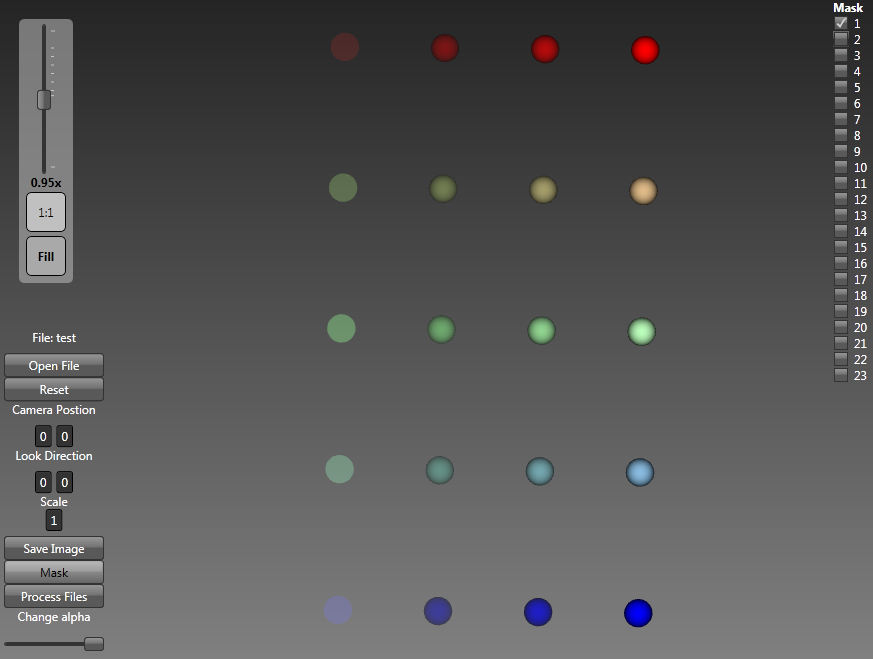
\includegraphics[scale=0.6]{test}
%	\caption{Zbi�r testowy 20 atom�w .}
%\end{figure}

%\newpage

\subsection{MainWindow}
\label{subsec:mainWindow}

W pliku MainWindow.cs znajduje si� kod, kt�ry definiuje interakcj� u�ytkownika z aplikacj�. Architektura WPF opiera si� na zdarzeniach, kt�re s� obs�ugiwane przez funkcje obs�ugi. W przypadku klasy MainWindow jest to 19 funkcji odpowiedzialnych za m.in. obs�ug� przycisk�w, powi�kszanie lub pomniejszanie modelu, zmian� kamery, zmian� wektora kierunkowego kamery, skalowanie, zapis zrzutu ekranu, zmian� maski, przetwarzanie grupy plik�w oraz zmian� prze�roczysto�ci. Typ MainWindow definiuje r�wnie� pola, kt�re opisuj� stan. Pierwszy z nich to lista obiekt�w typu Atom z pocz�tkow� pojemno�ci� dla 2000 element�w. Kolejna jest lista masek filtruj�ca serie pomiarowe. Nast�pnie obiekty typu AtomBuldier, MouseHelper, domy�lny promie� dla atom�w wynosz�cy 1.0 oraz �a�cuch znak�w wskazuj�cy u�ytkownikowi, �e �aden plik nie zosta� wybrany.

Funkcje klasy MainWindow mo�na podzieli� na 3 grupy: tworzenie modelu, modyfikacja parametr�w i przetwarzanie grupy modeli. Tworzenie modelu definiuje poni�szy algorytm:
\begin{enumerate}%[1)]
\item U�ytkownik naciska przycisk Open File i w oknie wyboru pliku wybiera plik danych z rozszerzeniem .chmc
\item Czytane s� dane z wybranego pliku, na podstawie kt�rych tworzona s� obiekty reprezentuj�ce atomy
\item Lista stworzonych atom�w jest filtrowana poprzez mask�
\item Tworzony jest model 3D
\end{enumerate}
Atomy filtrowana s� poprzez zapytanie LINQ. LINQ jest now� technologi�, opracowan� przez firm� Microsoft. Definiuje zbi�r metod, z kt�rych tworzone s� zapytania dla obiekt�w, takich jak kolekcje, bazy danych, XML czy inne zbiory danych. Jest to cz�� j�zyka, kt�ra bazuje na funkcjonalnym stylu programowania.\cite{csharp}. Zastosowa�em zapytanie LINQ do filtracji serii atom�w, kt�re s� zgodne z wybran� mask�.

\begin{lstlisting}
private void draw()
{
    var filteredAtoms = from atom in atoms
                        where masks.Contains(atom.PositionNumber)
                        select atom;
                        
    visualModel.Content = atomBuldier.CreateModel(filteredAtoms,
                                      alphaSlider.Value);
}
\end{lstlisting}
Czytelnik znaj�cy j�zyk SQL mo�e dostrzec podobie�stwo s��w kluczowych w zapytaniach LINQ.

Przetwarzanie grupy modeli jest w gruncie rzeczy modyfikacj� algorytmu dla pojedynczego modelu:
\begin{enumerate}%[1)]
\item Po naci�nieciu Process Files u�ytkownik, w oknie wyboru folderu, wybiera folder z plikami
\item Wczytywane s� pliki o rozszerzeniu .chmc
\item Dla ka�dego pliku wczytywane s� dane, filtrowane atomy zgodnie z mask�, renderowane i ustawiane s� parametry, kt�re zdefiniowa� u�ytkownik
\item Ka�dy model zapisany jest w pliku w formacie PNG, gdzie jego nazwa odpowiada temperaturze
\end{enumerate}
Poniewa� przetwarzanie du�ej liczby plik�w mo�e trwa� d�u�sz� chwil�, aplikacja wy�wietla kolejne modele, tak aby u�ytkownik wiedzia�, �e program nie zawiesi� dzia�ania. Dodatkowo na �rodku ekranu pojawia si� napis ,,Processing Files''.

\subsection{MouseHelper}
\label{subsec:mouseHelper}

Klasa MouseHelper s�u�y do obrotu obiektu przy u�yciu myszki. W tym celu WPF u�ywa kwaternion�w. Dla ka�dego ruchu myszki w poziomie i pionie obliczany jest obr�t obiektu, je�eli wci�ni�ty jest lewy klawisz a mysz znajduje si� w obr�bie okna.

%---------------------------------------------------------------------------

\section{Graficzny Interfejs U�ytkownika}
\label{sec:grafInter}

Graficzny interfejs u�ytkownika (ang. Graphical User Interface), nazywany r�wnie� �rodowiskiem graficznym, stanowi og�lne okre�lenie sposobu prezentacji informacji przez komputer oraz sposobu interakcji z u�ytkownikiem. G��wnym sposobem interakcji jest operacja na r�nych elementach, kt�re s� rysowane na monitorze pod postaci� obraz�w. Klasycznie u�ytkownik komunikuje si� z komputerem przy pomocy komend tekstowych\cite{GUIdef}.

Prekursorem wszystkich graficznych interfejs�w by� Sketchpad. Sketchpad zosta� stworzony z my�l� o wsparciu projekt�w technicznych. U�ytkownik przy pomocy specjalnego pi�ra tworzy� figury geometryczne, kt�rymi nast�pnie m�g� manipulowa� poprzez obr�t, skalowanie i przesuniecie. \cite{Sketch}

Pierwsze prototypu interfejs�w znanych z dzisiejszych system�w powsta�y w laboratorium PARC firmy Xerox. PARC User Interface zawiera� okienka, przyciski, ikony i menu. Dodano obs�ug� urz�dzenia wskazuj�cego poza standardow� klawiatur�. \cite{parc}

GUI mojej aplikacji sk�ada si� z g��wnego okna, w kt�rym wy�wietlane s� modele atom�w i dw�ch paneli bocznych.

\begin{figure}[h!]
  \centering
	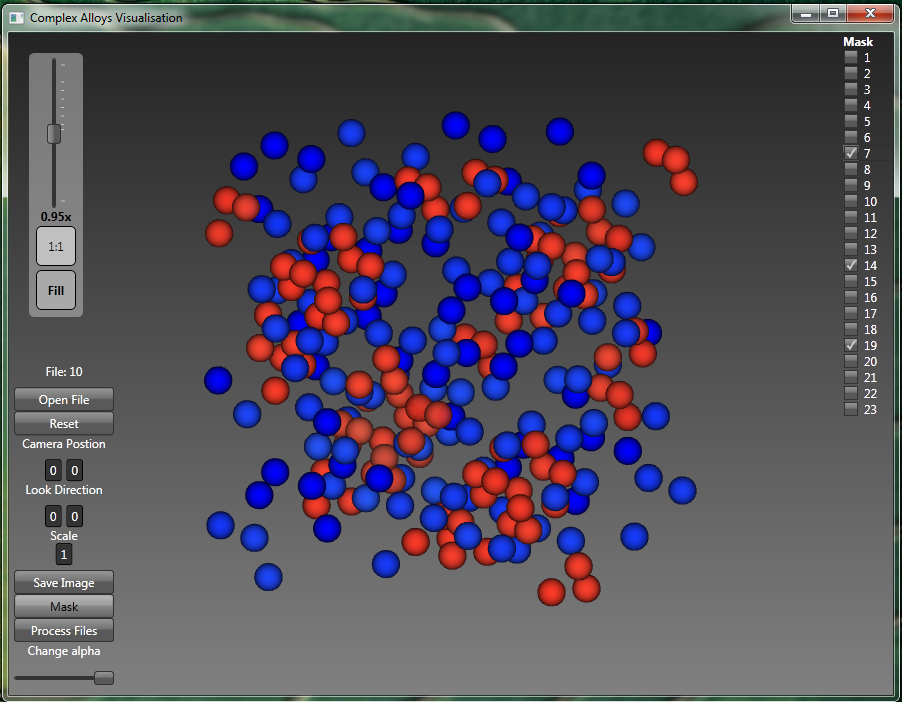
\includegraphics[scale=0.5]{gui}
	\caption{GUI programu do wizualizacji CMA.}
\end{figure}

%\newpage

W lewym panelu znajduje si� kontrolka odpowiedzialna za skalowanie modelu. 

\begin{figure}[h!]
  \centering
	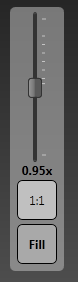
\includegraphics[scale=1.0]{zoom}
	\caption{Kontrolka skalowania modelu.}
\end{figure}

%\newpage

Atomy mog� by� skalowane od 0.01 do 100 przy u�yciu k�ka w myszce lub bezpo�rednio suwakiem. Kontrolka mo�e r�wnie� wr�ci� do domy�lnej skali 1:1 lub wype�ni� ca�y ekran. S�u�� do tego przyciski odpowiednio: ,,1:1'' oraz Fill.

W lewym panelu znajduj� si� r�wnie� elementy odpowiedzialne za g��wn� funkcjonalno�� aplikacji.

\begin{figure}[h!]
  \centering
	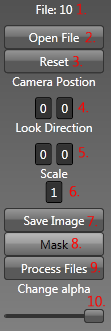
\includegraphics[scale=1.0]{lpanel}
	\caption{Lewy panel GUI.}
	\label{fig:lpanel}
\end{figure}

%\newpage

Rysunek \ref{fig:lpanel}: posiada ponumerowane kontrolki, kt�re odpowiednio s�u�� do:
\begin{enumerate}%[1)]
\item Wy�wietlania nazwy pliku, z kt�rego stworzony jest model
\item Otwierania pliku z modelem, kt�ry nast�pnie jest parsowany do tworzenia modelu
\item Powrotu do domy�lnych ustawie�
\item Zmiany pozycji kamery w p�aszczy�nie xy
\item Zmiany wektora, w jakim kierunku skierowana jest kamera

\item Skalowania promienia atom�w
\item Zapisu zrzutu ekranu
\item Otwierania i zamykania panelu masek
\item Przetwarzania grupy plik�w
\item Zmiany prze�roczysto�ci 
\end{enumerate}

Ka�dy z element�w panelu zosta� zaprojektowany w taki spos�b, aby rezultat operacji by� natychmiast widoczny dla u�ytkownika np. brak dodatkowego kroku w postaci od�wie�ania. Gdy u�ytkownik wpisze nieprawid�owe dane do pola tekstowego, tekst jest pod�wietlony kolorem czerwonym. Dane sprawdzane s� z ka�dym klikni�ciem klawiatury. 

Lewy panel zawiera kontrolki s�u��ce do filtracji atom�w. 
\begin{figure}[h!]
  \centering
	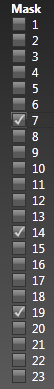
\includegraphics[scale=0.8]{rpanel}
	\caption{Maski serii atom�w.}
\end{figure}

Poprzez klikni�cie odpowiedniego checkboxa dodajemy lub usuwamy seri� atom�w.


%---------------------------------------------------------------------------

\section{Testy}
\label{sec:testy}

 Testowanie oprogramowania jest to badanie prowadzone w celu zapewnienia zainteresowanym stronom informacji o jako�ci produktu lub us�ugi. Testowanie mo�e r�wnie� dostarczy� dodatkowych informacji o systemie, takich jak ryzyko zwi�zanie z projektem. 
 
Testowanie oprogramowania mo�na podzieli� na proces weryfikacji i walidacji sk�adaj�cy si� z czterech cz�ci:
\begin{enumerate}%[1)]
\item sprawdzenie produktu pod k�tem wymaga�
\item czy oprogramowanie zachowuje si� zgodnie z przewidywaniami
\item czy mo�e by� zaimplementowane zgodnie z wymaganiami
\item czy spe�nia potrzeby zleceniodawcy
\end{enumerate}

Testowanie tradycyjnie jest jednym z ostatnich etap�w w budowaniu aplikacji, jednak nowe metodologie, takie jak Agile, przesuwaj� znaczn� cz�� test�w do pocz�tkowych etap�w.\cite{extest} 

Przyk�adem takiego podej�cia jest Test-driven development (TDD), kt�ry opiera si� na kr�tkich cyklach podzielonych na: 
\begin{enumerate}%[1)]
\item tworzenie automatycznych test�w pocz�tkowych, kt�re opisuj� now� funkcjonalno�� 
\item pisanie pocz�tkowego kodu, kt�ry "przechodzi" przez wszystkie testy
\item refactoring kodu do okre�lonych standard�w
\end{enumerate}
Programi�ci cz�sto korzystaj� z TDD, aby poprawi� jako�� istniej�cego ju� programu. \cite{TDD}

Testowanie oprogramowania nigdy nie potwierdzi w 100\% czy system nie ma wad, lecz daje nam odpowied� na inne pytanie: Czy w pewnych warunkach oprogramowanie posiada b��dy?

Przeanalizujmy poni�sz� funkcj�:
\begin{lstlisting}
int add(int a, int b) {
    return a + b;
}
\end{lstlisting}

Aby w pe�ni przetestowa� t� funkcj�, nale�y sprawdzi� wynik dla ka�dych mo�liwych danych wej�ciowych. W przypadku typu liczbowego int daje nam to 4 294 967 296 mo�liwo�ci dla pierwszej oraz tyle samo dla drugiej liczby. W sumie daje to $ 1,84467441 \times 10^{19}$ test�w jednostkowych tej trywialnej funkcji! Dlatego nigdy nie tworzy si� wszystkich mo�liwych test�w. Funkcj� add, w praktyce, nale�y przetestowa� dla kilku warto�ci losowych oraz dla przypadk�w szczeg�lnych, takich jak maksymalna warto�� int. \\
Bardzo wa�nym elementem testowania jest tworzenie test�w z uwzgl�dnieniem odbiorcy oprogramowania. U�ytkownicy gry video diametralnie r�ni� si� od u�ytkownik�w systemu bankowego. 

Testowanie oprogramowania jest z�o�onym procesem, kt�ry wymaga sporych nak�ad�w ludzkich. Jak zawsze w takich sytuacjach, pojawia si� pytanie o op�acalno�� prowadzenia test�w. W 2002 National Institute of Standards and Technology (NIST) sporz�dzi� raport dotycz�cy wp�ywu b��d�w oprogramowania na gospodark� ameryka�sk�. Roczny koszt nieprawid�owego dzia�ania aplikacji w roku 2002 wyni�s� 59,5 mld dolar�w. Oko�o jedn� trzeci� tej kwoty da si� zaoszcz�dzi�, je�eli oprogramowanie by�oby lepiej testowane\cite{reportEco}.
Wcze�niej wykryte b��dy s� ta�sze w naprawie. Potwierdza to analiza wielu projekt�w, kt�rej wyniki opisuje dana tabelka. Warto�ci reprezentuj� krotno�ci pojedynczego kosztu\cite{codeComplete}.


\begin{table}
    \centering
    \scalebox{0.8}{
    \begin{tabular}{|c|c|c|c|c|c|c|} 
        \hline
\multicolumn{2}{|c|}{Koszt naprawy} & \multicolumn{5}{|c|}{Czas wykrycia} \\ \cline{3-7}
    \multicolumn{2}{|c|}{} & Wymagania & Architektura  & Programowanie & Testy & Po dostarczeniu  \\ \hline
        Czas Wyst�pienia & Wymagania & 1x & 3x & 5-10x & 10x & 10-100x \\\cline{2-7} & Architektura                        		& -  & 1x  & 10x & 15x & 25-100x \\\cline{2-7} 
        & Programowanie  & - & - & 1x & 10x & 10-25x  \\\hline
    \end{tabular}
    }
    \caption{Zale�no�ci miedzy kosztem naprawy b��du a etapem wyst�pienia. }
\end{table}

Testowanie oprogramowania mo�na podzieli� na kilka kategorii. Jednym z nich jest podzia� na testy statyczne i dynamiczne. Testy statyczne s� to testy, kt�re nie wymagaj� uruchomienia programu np. Code Review, za� testy dynamiczne s� to takie, w kt�rych aplikacja jest uruchamiana np. testy jednostkowe.

Metody testowania r�wnie� dziel� si� na Black-box oraz White-box. Przy testowaniu typu White-box tester ma wiedz� o architekturze i wewn�trznej strukturze testowanego modu�u. Stosowane s� g��wnie jako testy jednostkowe, testy API. Testy typu Black-box nie korzystaj� z wewn�trznych informacji. Tester ma tylko informacj� o spodziewanym rezultacie. Istniej� r�wnie� hybrydowe metody, nazywane Grey-box.\cite{softTesting} 

Podczas tworzenia aplikacji do wizualizacji CMA korzysta�em g��wnie z test�w GUI, wydajno�ciowych i regresywnych. Testy GUI maj� na celu sprawdzenie dzia�ania ka�dego elementu interfejsu. Istotne nie tylko jest poprawne dzia�anie ka�dego z element�w, ale r�wnie� ich zachowanie w okre�lonej sekwencji. Z tego powodu wraz z komplikacj� GUI liczba test�w ro�nie eksponencjalnie. M�j program posiada tylko kilkana�cie element�w, dlatego manualne testowanie jest wystarczaj�ce.

Testy wydajno�ciowe maj� na celu zbadanie, jak system zachowuje si� pod obci��eniem. Mo�emy okre�li�, czy system spe�nia wymagania wydajno�ciowe, zbada� skalowalno�� i niezawodno��. Testy wydajno�ciowe mog� r�wnie� pom�c w wykrywaniu b��d�w. Podczas testowania odkry�em, �e jedna z metod zajmuje oko�o 95\% czasu. By� to banalny b��d. Dla ka�dego atomu oblicza�em siatk� na nowo, mimo �e jest wsp�dzielona.
Testy pomog�y r�wnie� zoptymalizowa� przetwarzanie grupy plik�w. W pierwszej wersji przetworzenie 30 plik�w zajmowa�o oko�o 20 minut. W ostatecznej wersji proces ten trwa oko�o 3 minuty.

Testy regresywne jest to rodzaj testowania, kt�ry szuka b��d�w w istniej�cej funkcjonalno�ci po wprowadzeniu zmian. Innymi s�owy, chcemy zbada�, czy wprowadzane poprawki nie naruszaj� dzia�aj�cej poprawnie cz�ci systemu.\cite{softTesting} Po ka�dej wi�kszej zmianie, a przed dodaniem kodu do systemu kontroli wersji, przeprowadza�em co najmniej jeden test regresywny.

Ostatnim testem by�a kontrola wizualizacji prawdopodobie�stw obsadzenia. Pos�u�y� do tego plik test.chmc, kt�ry zawiera� kombinacje obsadze� ze zmian� od ca�kowitego Al do ca�kowitego Mg poprzez obsadzenia mieszane. Generuje to w sumie 20 atom�w (rysunek \ref{fig:test}).

\begin{figure}[h!]
	\centering
	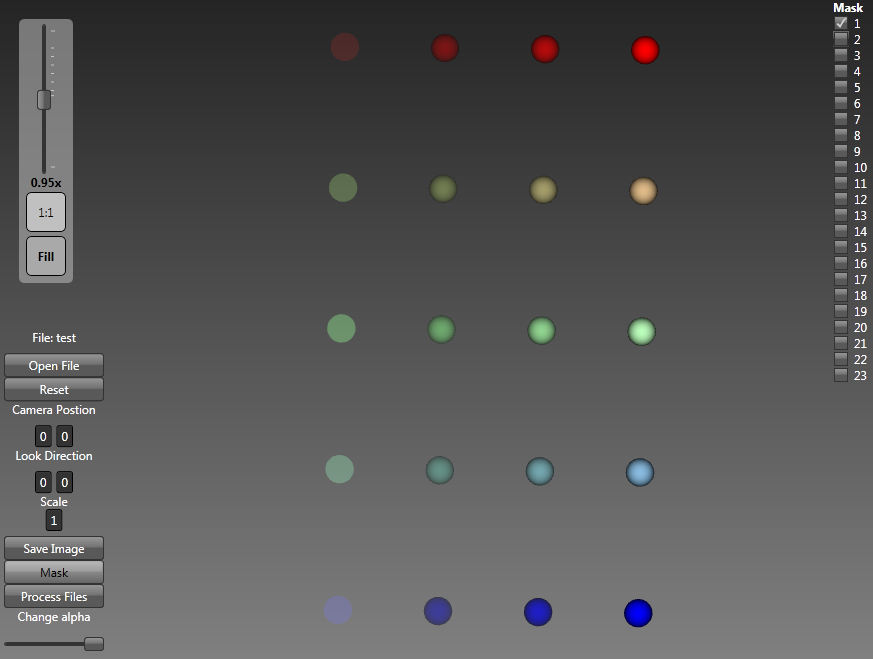
\includegraphics[scale=0.5]{test}
	\caption{Zbi�r testowy 20 atom�w.}
	\label{fig:test}
\end{figure}

Na rysunku \ref{fig:test} wida�, �e przej�cia w palecie s� g�adkie oraz kolor, zgodnie z oczekiwaniami, przechodzi od czerwonego do niebieskiego z domieszk� zielonej barwy.
\chapter{Podsumowanie}
\label{cha:podsumowanie}

W rozdziale zaprezentuj� wyniki, opisz� jak mo�na rozszerzy� aplikacj� oraz podsumuj� zrealizowane zadania.

%---------------------------------------------------------------------------
\section{Wyniki}
\label{sec:wyniki}

Celem pracy by�o stworzenie narz�dzia, dlatego postanowi�em zamie�ci� kilka obraz�w wynikowych ilustruj�cych mo�liwo�ci aplikacji. Przyk�adowe wyniki wykorzystane do prezentacji mo�liwo�ci aplikacji zosta�y otrzymane z symulacji przeprowadzonej w 31 temperaturach, stopniowo obni�anych z pocz�tkowych 2000K do 400K. W trakcie  symulacji obserwujemy najpierw porz�dkowanie obsadze� na pozycjach naro�nych klaster�w (pozycje nr
8, 21) pomi�dzy 2000 a 1200K, a nast�pnie obserwujemy dyfuzj� i porz�dkowanie obsadze� na pozycjach 
Al w klasterze (nr 8) w zakresie temperatur od 900 do 600K. Poni�sze rysunki ilustruj� zmiany zachodz�ce
w systemie poprzez zmiany kolor�w i przezroczysto�ci odpowiednich obiekt�w. U�ytkownik mo�e w ka�dej chwili wykona� zrzut ekranu oraz zmienia� parametry modelu (rysunki ~\ref{fig:3_14_19} i ~\ref{fig:res2}).  

\begin{figure}[h!]
  \centering
	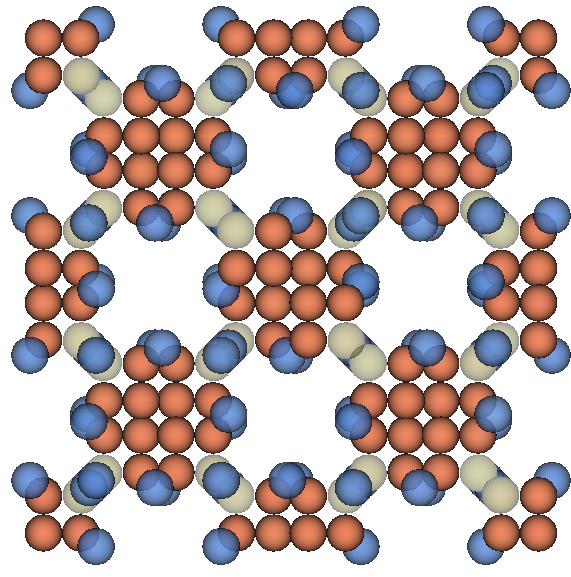
\includegraphics[scale=0.8]{res1}
	\caption{Seria pozycji nr 3, 14 i 19 atom�w $\beta$- Mg$_{2}$Al$_{3}$ przy temperaturze 2000K.}
	\label{fig:3_14_19}
\end{figure} 

\begin{figure}[h!]
  \centering
	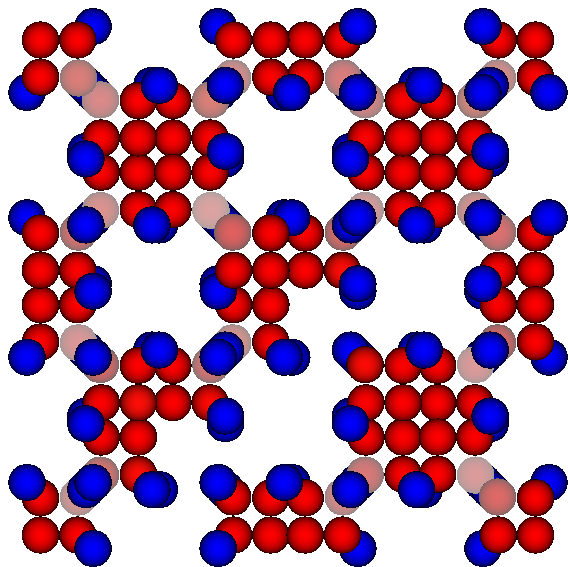
\includegraphics[scale=0.8]{res2}
	\caption{Seria pozycji 3, 14 i 19 atom�w $\beta$- Mg$_{2}$Al$_{3}$ przy temperaturze 400K.}
	\label{fig:res2}
\end{figure} 

%\begin{figure}[h!]
%  \centering
%	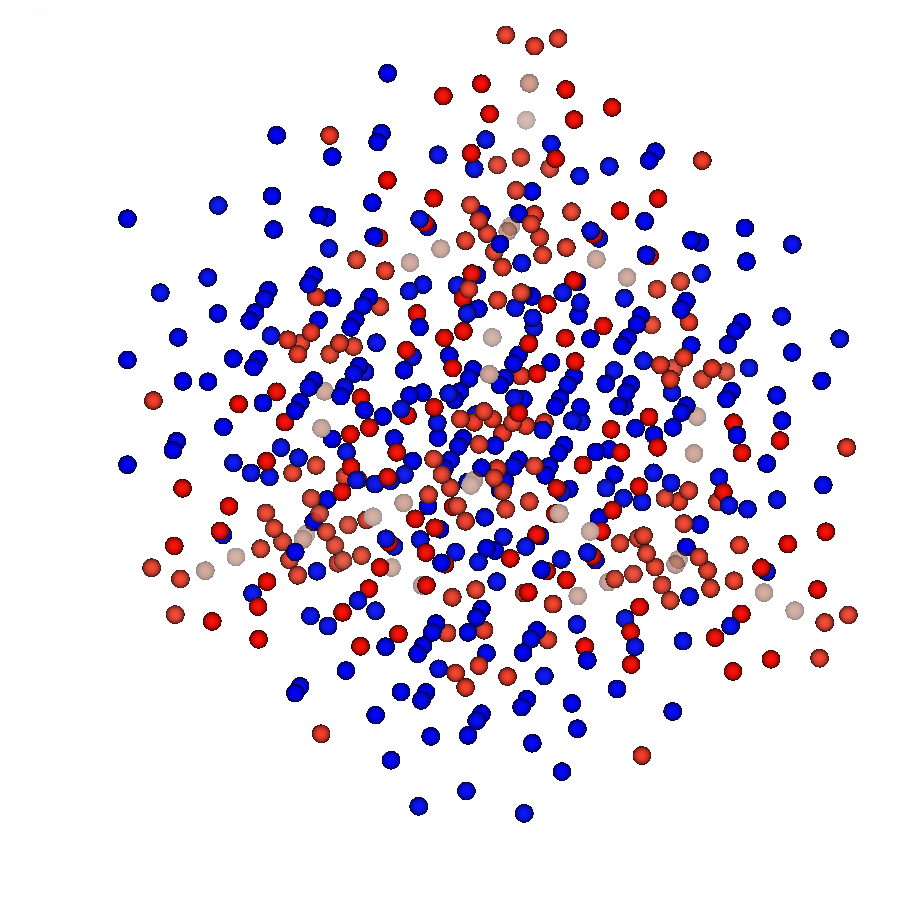
\includegraphics[scale=0.8]{res3}
%	\caption{Seria 1, 3, 4, 5, 7, 10, 14, 17, 20, i 22 atom�w $\beta$- Mg$_{2}$Al$_{3}$ przy temperaturze 1000K.}
%	\label{fig:res3}
%\end{figure} 

\clearpage
Przy przetwarzaniu wielu plik�w mo�emy stworzy� kolejne klatki przedstawiaj�ce ewolucj� systemu dla klastra g��wnego. Poni�ej kolejne stany pocz�wszy od temperatury 2000 K dla pozycji 1, 8, 11, 12, 13, 14, 21. Wszystkich modeli jest 31, dlatego zaprezentuj� tylko kluczowe klatki.

\begin{table}[ht]
\begin{minipage}[b]{0.48\linewidth}
\centering
	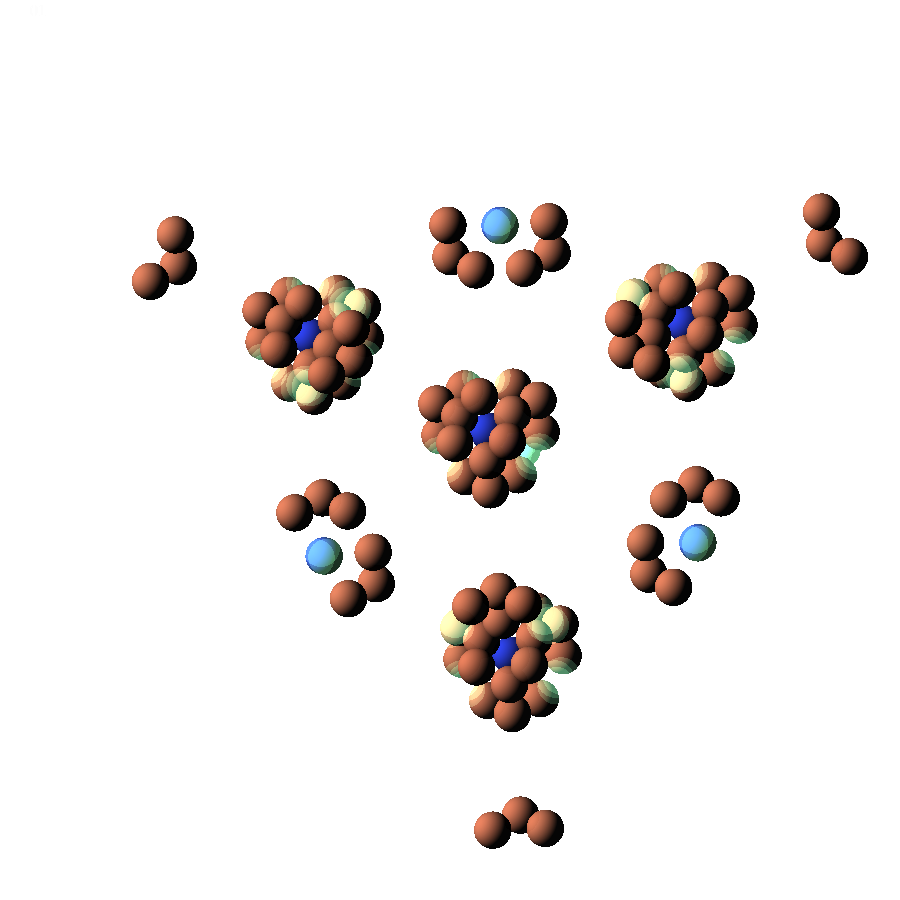
\includegraphics[scale=0.6]{01}
	\captionof{figure}{Stan kom�rki elementarnej dla temperatury 2000K.}
\end{minipage}
\hspace{0.5cm}
\begin{minipage}[b]{0.48\linewidth}
\centering
	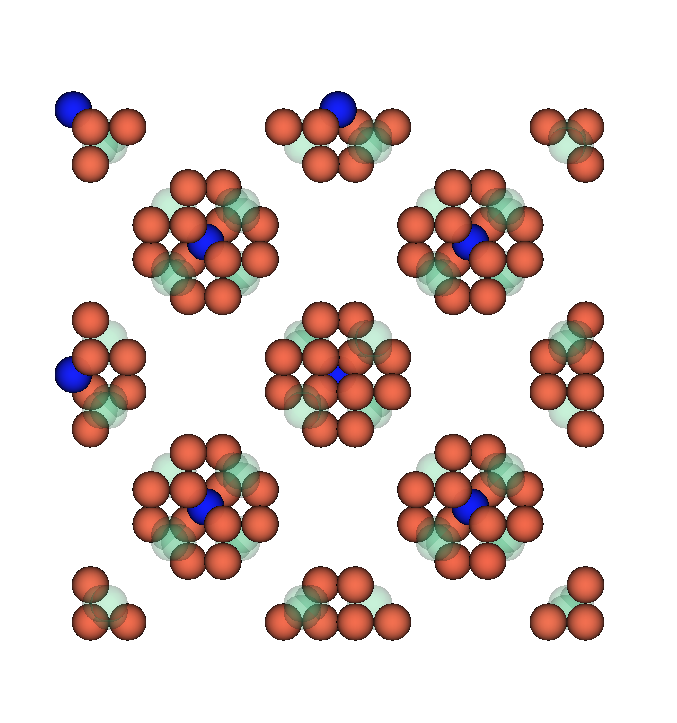
\includegraphics[scale=0.6]{02}
	\captionof{figure}{Stan kom�rki elementarnej dla temperatury 1500K.}
\end{minipage}
\end{table}

\begin{table}[ht]
\begin{minipage}[b]{0.48\linewidth}
\centering
	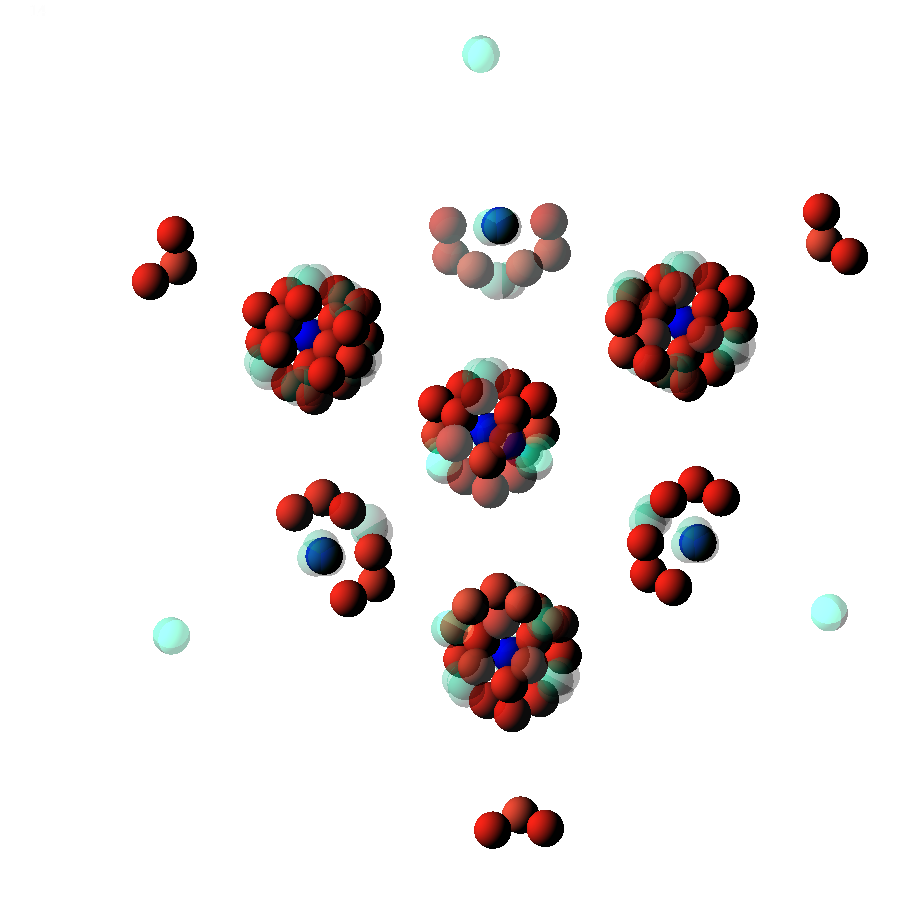
\includegraphics[scale=0.6]{14}
	\captionof{figure}{Stan kom�rki elementarnej dla temperatury 900K.}
\end{minipage}
\hspace{0.5cm}
\begin{minipage}[b]{0.48\linewidth}
\centering
	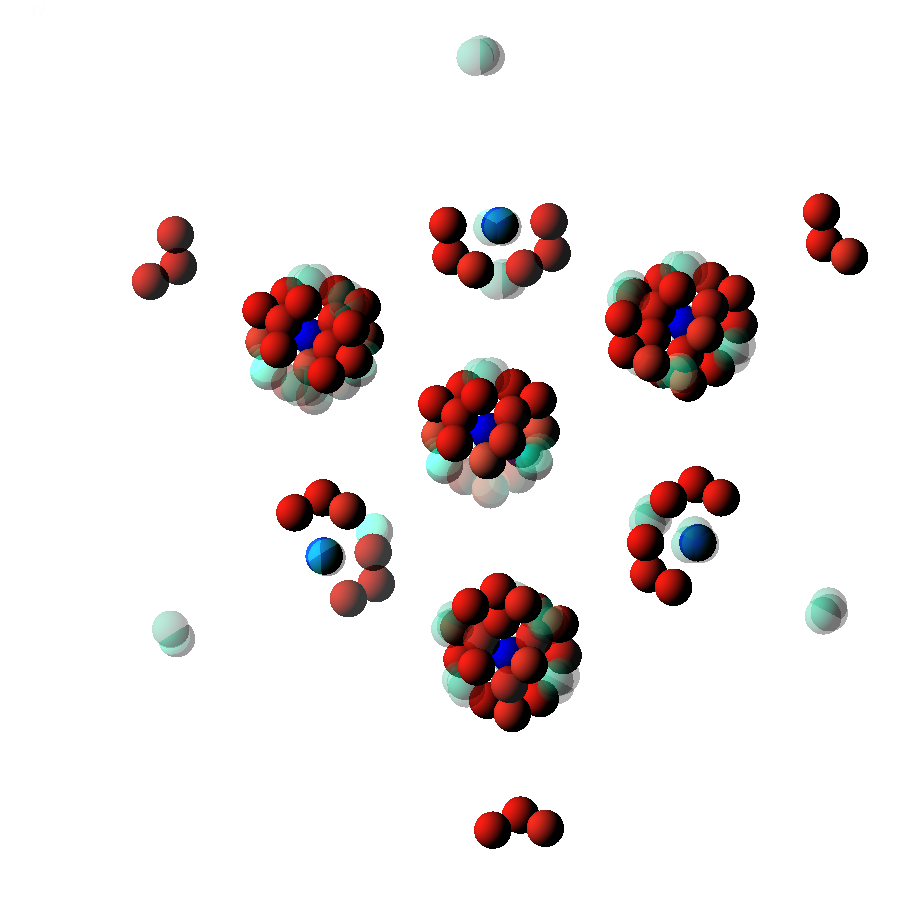
\includegraphics[scale=0.6]{17}
	\captionof{figure}{Stan kom�rki elementarnej dla temperatury 850K.}
\end{minipage}
\end{table}

\begin{table}[ht]
\begin{minipage}[b]{0.48\linewidth}
\centering
	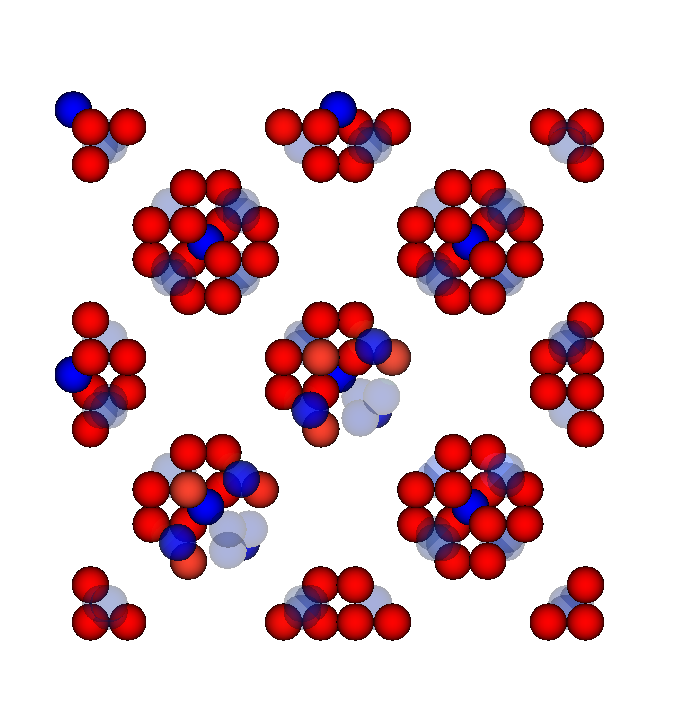
\includegraphics[scale=0.6]{25}
	\captionof{figure}{Stan kom�rki elementarnej dla temperatury 650K.}
\end{minipage}
\hspace{0.5cm}
\begin{minipage}[b]{0.48\linewidth}
\centering
	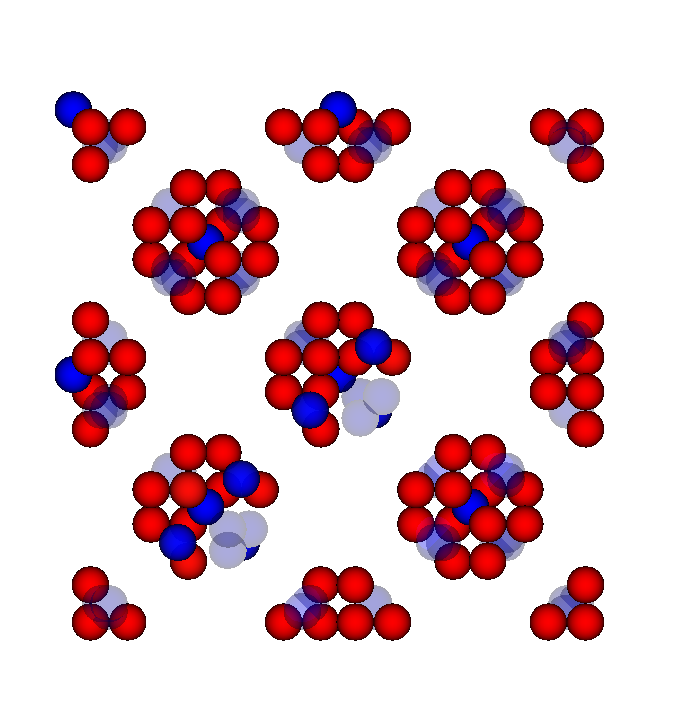
\includegraphics[scale=0.6]{31}
	\captionof{figure}{Stan kom�rki elementarnej dla temperatury 400K.}
\end{minipage}
\end{table}

\clearpage

Kolejna seria rysunk�w przedstawia po��czenia dla pozycji 3, 9, 10, 18 i 19.
%-----------------------
\begin{table}[ht]
\begin{minipage}[b]{0.48\linewidth}
\centering
	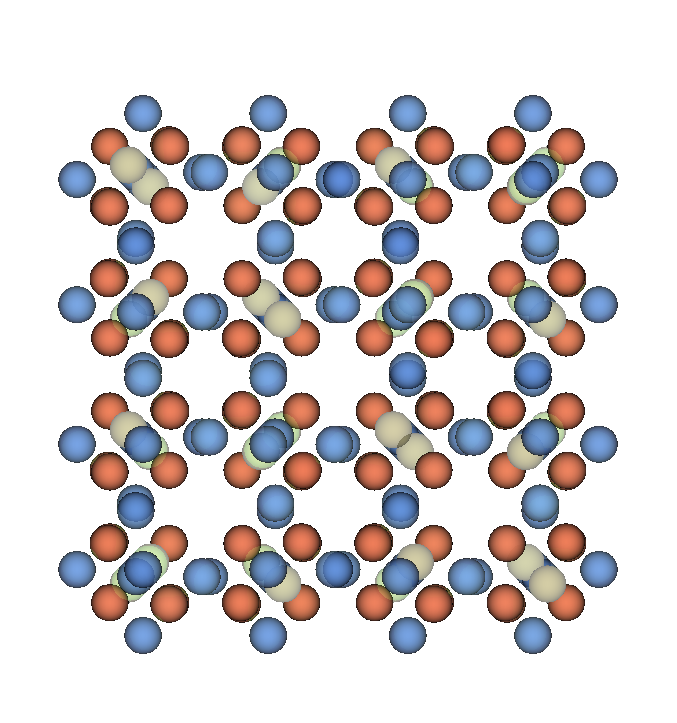
\includegraphics[scale=0.6]{201}
	\captionof{figure}{Stan kom�rki elementarnej dla temperatury 2000K.}
\end{minipage}
\hspace{0.5cm}
\begin{minipage}[b]{0.48\linewidth}
\centering
	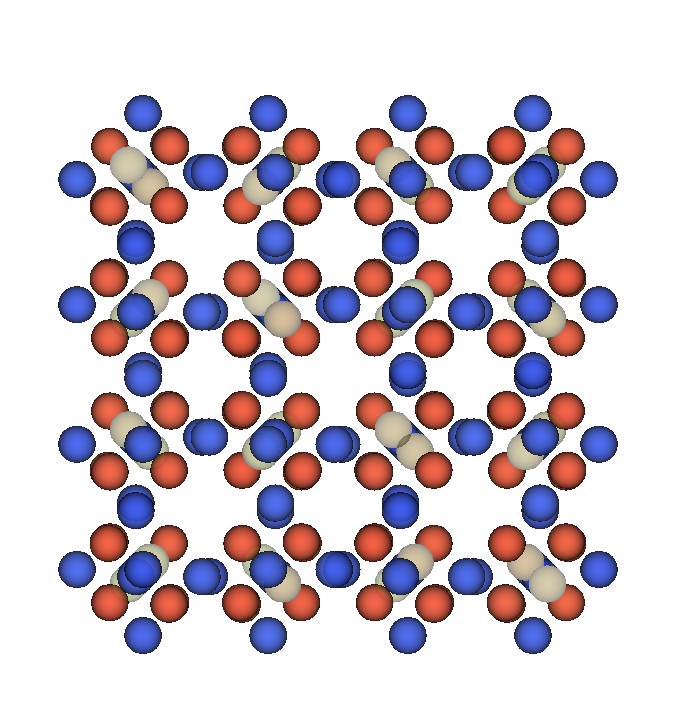
\includegraphics[scale=0.6]{202}
	\captionof{figure}{Stan kom�rki elementarnej dla temperatury 1500K.}
\end{minipage}
\end{table}

\begin{table}[ht]
\begin{minipage}[b]{0.48\linewidth}
\centering
	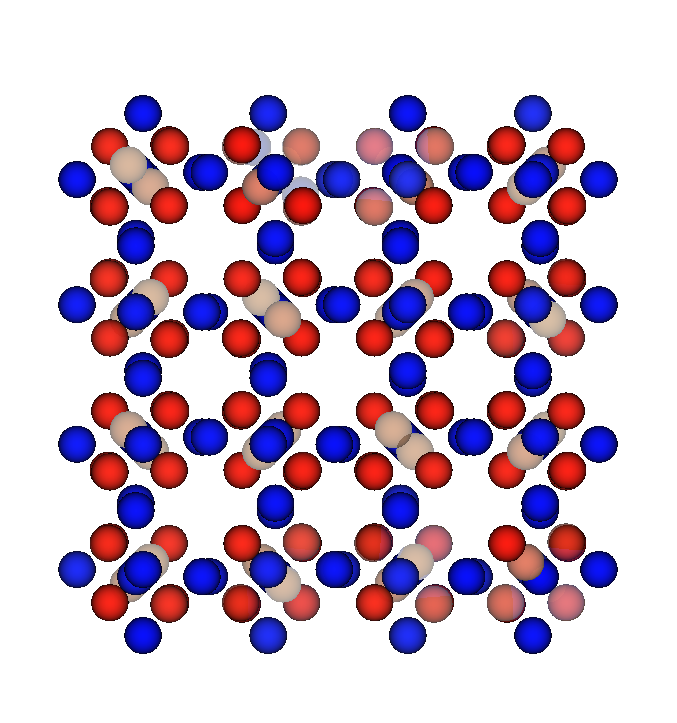
\includegraphics[scale=0.6]{214}
	\captionof{figure}{Stan kom�rki elementarnej dla temperatury 900K.}
\end{minipage}
\hspace{0.5cm}
\begin{minipage}[b]{0.48\linewidth}
\centering
	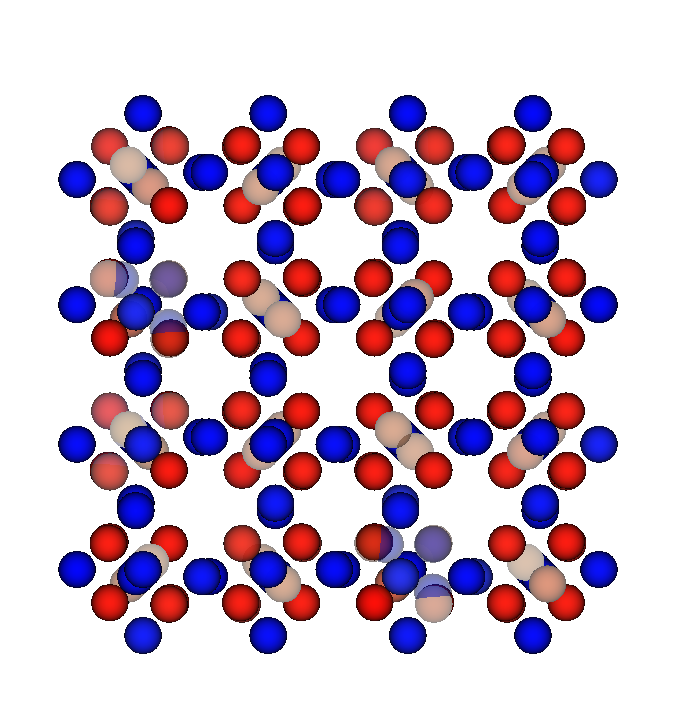
\includegraphics[scale=0.6]{217}
	\captionof{figure}{Stan kom�rki elementarnej dla temperatury 850K.}
\end{minipage}
\end{table}

\begin{table}[ht]
\begin{minipage}[b]{0.48\linewidth}
\centering
	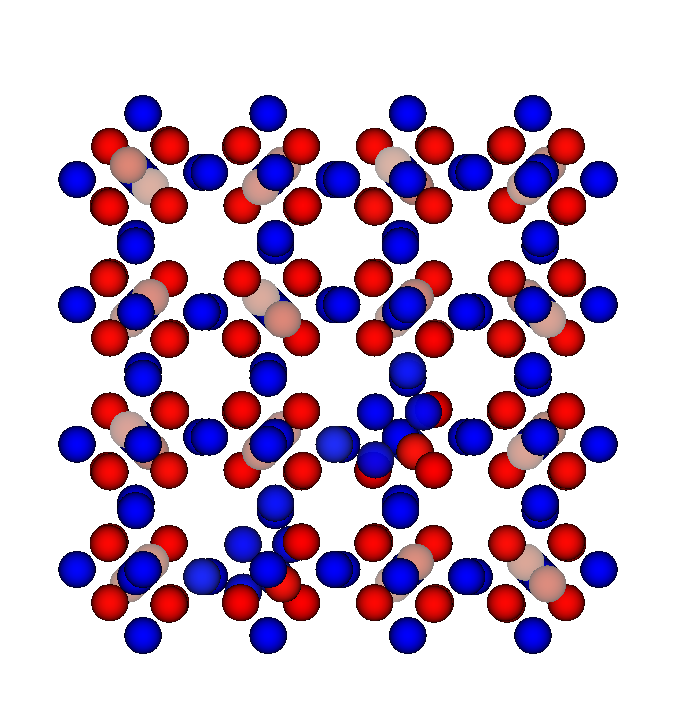
\includegraphics[scale=0.6]{225}
	\captionof{figure}{Stan kom�rki elementarnej dla temperatury 650K.}
\end{minipage}
\hspace{0.5cm}
\begin{minipage}[b]{0.48\linewidth}
\centering
	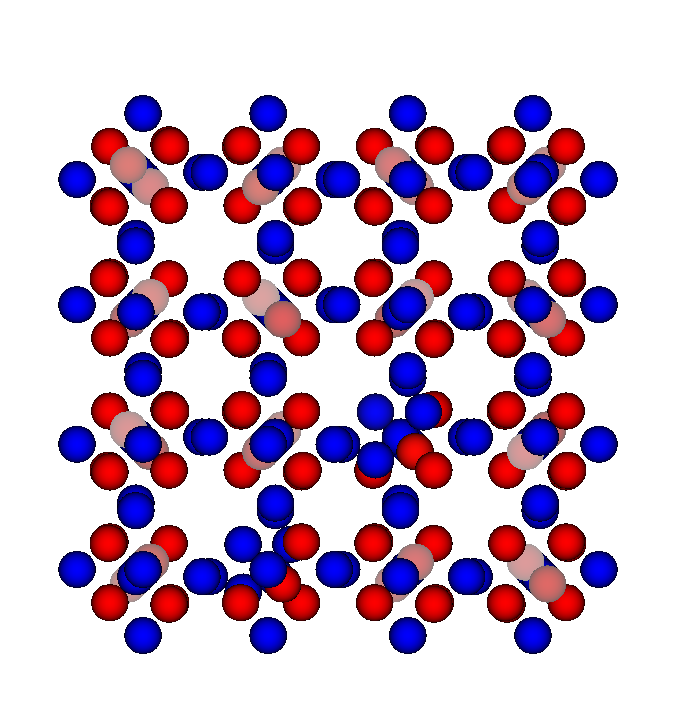
\includegraphics[scale=0.6]{231}
	\captionof{figure}{Stan kom�rki elementarnej dla temperatury 400K.}
\end{minipage}
\end{table}


\clearpage

Z obraz�w wynikowych z�o�y�em film. Mo�na go obejrze� pod adresem: http://www.youtube.com/watch?v=CsOJeIbpqro (wymagana jest przegl�darka z obs�ug� HTML5 lub z wtyczk� Flash).

\section{Mo�liwe rozszerzenia}
\label{sec:mozliweRoz}

Projekt znajduje si� po adresem http://alloysvisualisation.codeplex.com/. Posiada on w pe�ni otwarte �r�d�a na licencji New BSD. Ka�dy mo�e zmodyfikowa� aplikacje wed�ug w�asnych potrzeb. Program mo�e w bardzo �atwy spos�b zosta� zmieniony, tak aby wy�wietla� inny rodzaj modeli 3D. Naj�atwiej modyfikowa� program przy u�yciu Visual Studio 2010. Mo�liwa jest r�wnie� kompilacja z linii polece�. Do modyfikacji, poza �r�d�ami, niezb�dna jest r�wnie� biblioteka WPFExtension. Mo�na j� znale�� na stronie projektu.

%---------------------------------------------------------------------------
\section{U�yte narz�dzia i biblioteki}
\label{sec:uz}

Podczas implementacji korzysta�em z nast�puj�cych narz�dzi i bibliotek:
\begin{enumerate}%[1)]
\item �rodowisko programistyczne - Visual Studio 2010 Ultimate
\item �rodowisko uruchomieniowe - .Net 4.0
\item J�zyk C\# w wersji 4.0
\item System kontroli wersji - Team Foundation Server w serwisie codeplex.com
\item Biblioteka WPFExtensions - http://wpfextensions.codeplex.com/
\item Python 2.7
\end{enumerate}

\section{Zako�czenie}
\label{sec:zakonczenie}

Celem pracy by�o zaprojektowanie i implementacja systemu pozwalaj�cego na wizualizacje proces�w dyfuzji i porz�dkowania w stopach mi�dzymetalicznych, takich jak stop $\beta$- Mg$_{2}$Al$_{3}$. Kluczowe by�y dwa elementy: Przedstawienie modelu siatki krystalicznej z mo�liwo�ci� wygodnej manipulacji obiektami oraz przetwarzanie grupy plik�w, aby wyniki pokazywa�y ewolucj� systemu.

Interfejs jest �atwy i intuicyjny w u�yciu. Po�o�y�em spory nacisk na wydajno�� aplikacji. U�ytkownik widzi niemal natychmiast rezultat ka�dej operacji, dlatego wyb�r technologii mia� spore znaczenie. Wybra�em j�zyk C\# dzia�aj�cy w ramach technologii .Net. W tym przypadku daje on optymalne rozwi�zanie pomi�dzy sprawno�ci� programowania, a szybko�ci� dzia�ania. Jako �rodowisko programistyczne, ze wzgl�du na najlepsze wsparcie, wybra�em Visual Studio 2010 Ultimate.

W Pierwszym etapie pracy skupi�em si� na zebraniu wymaga� projektowych. Temat z�o�onych stop�w metalicznych (CMA) by� dla mnie nowy, dlatego pomoc merytoryczna promotora okaza�a si� niezwykle cenna. W kolejnym etapie stworzy�em odpowiednie prototypy, aby wybra� najlepsz� z technologii. W ostatnim etapie zaprojektowa�em i zaimplementowa�em aplikacj�, kt�r� nast�pnie przetestowa�em.

Cel pracy zosta� osi�gni�ty. Aplikacja do wizualizacji proces�w zachodz�cych w z�o�onych stopach metalicznych jest w pe�ni funkcjonalna zgodnie ze specyfikacj�. Interfejs graficzny jest prosty w obs�udze. Program z powodzeniem mo�e by� zastosowany do innych cel�w, nawet bez ingerencji w kod.


%---------------------------------------------------------------------------










% itd.
 \appendix
 \chapter{Instrukcja obs�ugi}
\label{cha:insObs}

%---------------------------------------------------------------------------
\section{Pobieranie aplikacji}
\label{sec:oobieranieAplikacji}

Aplikacje nale�y pobra� ze strony alloysvisualisation.codeplex.com (po prawej stronie znajduje si� przycisk Download). W skompresowanym pliku znajduje si�:
\begin{enumerate}%[1)]
\item Plik wykonywalny ComplexAlloysVisualisation.exe
\item skrypt chmcMergeScript.py
\item biblioteka WPFExtensions.dll
\item folder out
\end{enumerate}

Plik ComplexAlloysVisualisation.exe startuje aplikacj�. 

\section{Tworzenie modelu i manipulacja}
\label{sec:modelManipulacja}

Po uruchomieniu aplikacji nale�y nacisn�� przycisk Open File i wybra� plik .chmc. W folderze out znajduje si� klika przyk�adowych plik�w. Aplikacja domy�lnie stworzy model z serii 14. Aby zmieni� serie, nale�y nacisn�� przycisk Mask i w panelu po prawej stronie wybra� interesuj�ce nas serie.  W rozdziale 4.3 Graficzny Interface U�ytkownika znajduje si� dok�adny opis ka�dej funkcjonalno�ci.

\section{Przetwarzanie grupy plik�w}
\label{sec:przetwarzanie}

W celu przetworzenia grupy plik�w, nale�y uruchomi� aplikacje i nacisn�� przycisk Process Files. Po naci�ni�ciu pojawi si� okno, gdzie nale�y wybra� folder z plikami .chmc.

\begin{figure}[h!]
  \centering
	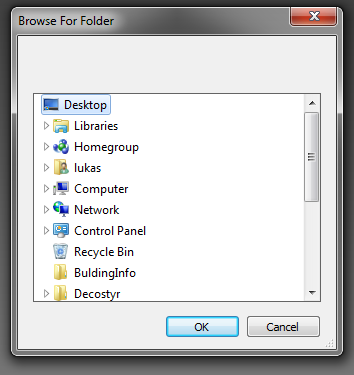
\includegraphics[scale=0.6]{process}
	\caption{Okno wyboru folderu.}
\end{figure}

\newpage

Przetwarzanie plik�w przy kliku seriach powinno trwa� oko�o 0,6 s dla ka�dego pliku. Wyniki zapisane zostan� w folderze screens. 


% \include{dodatekB}
% itd.

\listoffigures
\listoftables

\bibliographystyle{plain}
\bibliography{bibliografia}


\end{document}
